\chapter{The Arabic Script}
\label{ch:arabic}
\thispagestyle{empty}
\newpage
\refsection

The Arabic writing system is one of the geographically and chronologically most
widely used writing system in human history. It is the primary script for the
Arabic language, Farsi, Urdu, and multiple others on the Indian subcontinent
and has been used historically to produce texts in Spanish to Chinese.

While there is still some dispute on its exact origins, the scholarly consensus
is that the Arabic script evolved either from Nabatean or Syriac script in the
Middle East over the course of multiple centuries with maturation occuring
during the seventh century CE.  Linked closely to the spread of Islam, a number
of alphabetic variants and calligraphic regional styles developed in the
subsequent centuries. Nevertheless it is far from a purely liturgical script
with a wealth of administrative records, philosophical and scientific
treatises, poetry, \dots existing.

It is therefore of a misnomer to speak of a single Arabic script from the
perspective of DIA research. Persian epics in \emph{nastaʿliq} style on highly
decorated marbled paper have little in common with \emph{naskh} private
correspondence or the angular rectilinear writing of early \emph{kufic} quranic
codices. Each style in combination with the regional preferences and the
context of their utilization presents particular challenges. 

\section{The Principles of the Arabic Writing System}

The Arabic script is an \emph{abjad}, a consonantal writing system. Like
scripts for other semitic languages it only requires that consonants and long
vowels to be written, the reader is supposed to supply the appropriate short
vowels themselves from the context. Short vowels and other marks for features
such as doubling (gemination) and nunation (adding a final n), can optionally
be added (\emph{tashkīl}) but are only systematically used when transcribing
the \emph{qurʼān} or elementary texts for language learners. Like Syriac and
Hebrew it is written from right to left with the exception of numbers which are
written from left to right.

\begin{table}[!htbp]
\begin{minipage}{\textwidth}
\begin{center}
\caption{The 28 letters of the Arabic abjad}
\label{tab:abjad}
\renewcommand*{\thefootnote}{\alph{footnote}}
\begin{tabularx}{\textwidth}{XXXXXp{2.6cm}} \toprule
\textbf{isolated} & \textbf{initial} & \textbf{medial} & \textbf{final} & \textbf{name} & \textbf{transliteration}\\
\midrule
\textarabic{ا} & \textarabic{ا} & \textarabic{ـا} & \textarabic{ـا} & ʾalif & ā\\
\textarabic{ب} & \textarabic{بـ} & \textarabic{ـبـ} & \textarabic{ـب} & bāʾ & b\\
\textarabic{ت} & \textarabic{تـ} & \textarabic{ـتـ} & \textarabic{ـت} & tāʾ & t\\
\textarabic{ث} & \textarabic{ثـ} & \textarabic{ـثـ} & \textarabic{ـث} & thāʾ & th\\
\textarabic{ج} & \textarabic{جـ} & \textarabic{ـجـ} & \textarabic{ـج} & jīm & j\\
\textarabic{ح} & \textarabic{حـ} & \textarabic{ـحـ} & \textarabic{ـح} & ḥāʾ & ḥ\\
\textarabic{خ} & \textarabic{خـ} & \textarabic{ـخـ} & \textarabic{ـخ} & khāʾ & kh\\
\textarabic{د} & \textarabic{د} & \textarabic{ـد} & \textarabic{ـد} & dāl & d\\
\textarabic{ذ} & \textarabic{ذ} & \textarabic{ـذ} & \textarabic{ـذ} & dhāl & dh\\
\textarabic{ر} & \textarabic{ر} & \textarabic{ـر} & \textarabic{ـر} & rāʾ & r\\
\textarabic{ز} & \textarabic{ز} & \textarabic{ـز} & \textarabic{ـز} & zayn & z\\
\textarabic{س} & \textarabic{سـ} & \textarabic{ـسـ} & \textarabic{ـس} & sīn & s\\
\textarabic{ش} & \textarabic{شـ} & \textarabic{ـشـ} & \textarabic{ـش} & shīn & sh\\
\textarabic{ص} & \textarabic{صـ} & \textarabic{ـصـ} & \textarabic{ـص} & ṣād & ṣ\\
\textarabic{ض} & \textarabic{ضـ} & \textarabic{ـضـ} & \textarabic{ـض} & ḍād & ḍ\\
\textarabic{ط} & \textarabic{طـ} & \textarabic{ـطـ} & \textarabic{ـط} & ṭāʾ & ṭ\\
\textarabic{ظ} & \textarabic{ظـ} & \textarabic{ـظـ} & \textarabic{ـظ} & ẓāʾ & ẓ\\
\textarabic{ع} & \textarabic{عـ} & \textarabic{ـعـ} & \textarabic{ـع} & ʿayn & ʿ\\
\textarabic{غ} & \textarabic{غـ} & \textarabic{ـغـ} & \textarabic{ـغ} & ghayn & gh\\
\textarabic{ف} & \textarabic{فـ} & \textarabic{ـفـ} & \textarabic{ـف} & fāʾ & f\\
\textarabic{ق} & \textarabic{قـ} & \textarabic{ـقـ} & \textarabic{ـق} & qāf & q\\
\textarabic{ك} & \textarabic{كـ} & \textarabic{ـكـ} & \textarabic{ـك} & kāf & k\\
\textarabic{ل} & \textarabic{لـ} & \textarabic{ـلـ} & \textarabic{ـل} & lām & l\\
\textarabic{م} & \textarabic{مـ} & \textarabic{ـمـ} & \textarabic{ـم} & mīm & m\\
\textarabic{ن} & \textarabic{نـ} & \textarabic{ـنـ} & \textarabic{ـن} & nūn & n\\
\textarabic{ه} & \textarabic{هـ} & \textarabic{ـهـ} & \textarabic{ـه} & hāʾ & h\\
\textarabic{و} & \textarabic{و} & \textarabic{ـو} & \textarabic{ـو} & wāwʾ & w/ū\\
\textarabic{ي} & \textarabic{يـ} & \textarabic{ـيـ} & \textarabic{ـي} & yāʾ & y/ī\\
%\multicolumn{5}{c}{\textbf{vowel and diacritical marks}}\\
%\midrule
%\textbf{letter} & & & & \textbf{name} & \textbf{transliteration}\\
%\textarabic{َ} & & & & fatḥah & a\\
%\textarabic{ُُ} & & & & ḍammah & u\\
%\textarabic{ِ} & & & & kasrah & i\\
%\textarabic{ْ} & & & & sukūn & zero-vowel\\
%\textarabic{ّ} & & & & shaddah & doubled consonant\\
%\textarabic{ًٌ/ً/ٍ}& & & & tanwīn & nunation marks\\
%\textarabic{ء}  &  & & & hamzah\footnote{\emph{Hamzah} is not considered as one of the canonical 28 letters but can nevertheless occur isolated and notsolely as an diacritic.}  & ʾ\\
\bottomrule
\end{tabularx}
\end{center}
\renewcommand\footnoterule{}
\end{minipage}
\end{table}

The original abjad used for writing Classical Arabic with its twenty-eight
distinctive phonemes contains only eighteen graphemes \emph{rasm}, causing the
same grapheme to represent up to five different phonemes. bāʾ, tāʾ, thāʾ, nūn,
and yāʾ share the same shape and are, depending on their position in the word,
written the same way. These glyphs are distinguished by dots placed above or
below them: one below for bāʾ, two above for tāʾ, three above for thāʾ, one
above for nūn, and two below for yāʾ. Correspondingly, dots are used to
differentiate ghayn and ʼayn, ṣād and ḍād, and jīm, ḥāʾ, and khāʾ. In contrast
to vocalization dotting is mandatory and is present in all but the earliest
Arabic texts. See table~\ref{tab:abjad} for an overview of 

Arabic distinguishes itself from other widely used scripts like Latin,
Cyrillic, or Greek by the lack of a printed form, i.e. a form where letters are
written separately, and only the cursive form exists, albeit a large number of
styles exist. Like cursive forms of other scripts, individual letters change
their shape depending on their position in a word: initial, medial, final, and
independent shapes exist, in addition to more complex placement rules along the
baseline in relation to the adjacent letters. Contrary to the cursive forms of
Latin not all letters can be connected to their previous and following letters,
roughly one fifth do not connect to the following letter. As white space
therefore does not necessarily indicate the beginning of a new word,
calligraphers are largely free to vary inter-word, inter-syllable, and
inter-stroke spacing as desired. On the extreme end, a kind of \emph{scripta
continua} arrises\cite[pg. 15]{blair2006islamic}, abandoning word separation
completely, but even conventional calligraphic practice displays some amount of
spacing variation that can throw off optical character recognition systems.

Unlike many other scripts, Arabic does not know capital and lower case letter
forms and texts produced before the twentieth century CE do not contain
Western-style punctation or layout such as commas, periods, question marks,
paragraphs, \dots Instead particular words and phrases are used to introduce a
new sentence or question, strokes are placed above titles and headings, and a
variety of verse marks and signs aiding in recitation are used in Quranic
manuscripts after the ninth century CE \cite{awad2015evolution}.

The script has been adapted for a fairly large number of other languages, most
prominently Persian and Turkish that do have some additional phonemes. Letter
forms are usually adapted by adding dots to graphemes representing similar
phonemes in Arabic, e.g. the Persian \emph{pe} is derived from \emph{bāʾ} by
writing two additional dots below. Sometimes graphemes were also modified more
directly such as the letter \emph{gāf} which is written by adding another bar
above the letter \emph{kāf}. Similar transformations exist for other languages
with some such as \emph{xiao'erjing}, the writing of sinitic languages in
Arabic script, changing it into a full alphabet by making the marking of short
vowels mandatory or creating additional letters for short vowels. The Unicode
standard alone lists more than a hundred additional graphemes for local
variants of the Arabic script.

\subsection{Text Justification}

As described Arabic does not share many features with other alphabetic scripts
but none of these are a fundamental obstacle to a modern OCR pipeline.  While
the cursive nature was seen as a major hindrance to older methods based on
character classifiers which require accurate segmentation to the character
level, newer segmentation-less methods are largely unaffected by this.
Nevertheless the variability in spacing, even on machine-printed text, is still
the primary source of errors (see section~\ref{s:whitespace}). Unfortunately,
the bundle of techniques employed to justify text, i.e. measures ensuring that
text ends flush with the left end of the writing space, require methods aware
of their function in all parts of the OCR pipeline.

These arose from the proscription of hyphenation, the splitting of words to
facilitate line-wrapping, since the tenth century CE, as justification by
white space alone often results in a visually unpleasing result, a phenomenon
known as rivers in Western typography. Western-style hyphenation is thus only
present in some early Koran manuscripts, albeit without explicit splitting
markers such as hyphens. The most probable reason for its abandonment is the
relatively large impact on legibility, especially when the second fragment of a
word is continued on the subsequent page.

A technique popular with later calligraphers for hanging styles such as the
Persian \emph{nastaʼliq}, in particular for poetry written in hemistichs, is
the stacking or heaping of the last syllable or penstroke above the left end of
the line. This technique is particularly attractive for the Persian language
as many words end in the same letters resulting in negligible impact on
legibility. Similar stacking could be performed inside a line by changing the
location and size of diacritical marks \cite[pg. 14]{blair2006islamic}.

Similarly challenging to OCR systems are dislocated fragments into the margin.
Instead of heaping the last syllable on top of the previous stroke, it is
placed in the margin of a text, similarly to a marginal note. These two
practices add another dimension of complexity to the layout analysis component
of an OCR pipeline. First, the layout analysis system has to be able to
accurately detect these fragments, which the methods presented in
part~\ref{part:la} are certainly capable of, at least with models specifically
trained for the purpose. Secondly, these fragments have to be distinguished
from bona fide marginalia and interlinear notes or translations to be properly
inserted in the flow of text in the output by a reading order determination
algorithm that is aware of their existence. A naïve algorithm assuming text is
ordered from top to bottom will, even if other notes are correctly filtered
through previous classification by the segmenter, insert the fragment before
the text of the line it is associated with, i.e. reverse the order.
Unfortunately, reading order determination is a notoriously under-researched
task in DIA, and although some tentative approaches, such as
\cite{dejean2019versatile} that could serve as a basis for versatile reading
order determination methods, exist, all practically available OCR system
operate on simple heuristics.

Two more practices exist, although their impact on OCR performance should be
modest in most cases. The stretching of the letter body or the connections
between individual letters, interchangeably known as either \emph{taṭwīl} or
\emph{kashida}, although the latter term is reserved in some publications on
typography for the first technique. These are used in most Arabic styles,
albeit their exact placement differs between scripts, not only for
justification but also general highlighting of verse beginnings, heading, etc. 

The second consists of upward curving of the baseline, trading horizontal with
vertical space. For conventional layout analysis methods modelling lines as
either rectangular bounding boxes or undirected\footnote{Undirected in the
sense that there is no definition of the text orientation or direction
contained within the polygon but only a bounding polygon is given.} polygons,
these lines, as slanted lines in general, will often cause a degradation of
results. This can be linked to other lines protruding into the bounding box or
height normalization resulting in insufficient text size as demonstrated in
figure XX. Segmenters founded on the baseline paradigm, like the ones presented
in chapters~\ref{ch:icfhr,ch:hip}, do not suffer from this problem as they
allow projecting arbitrarily shaped lines onto a straight line.

\section{Supports and Production}

A consideration often overlooked in the OCR research community is the question
of supports. While the unique challenges of processing inscriptions in stone or
clay tablets are evident, subtle differences on supple writing surfaces are
usually disregarded. Papyrus and parchment being utilized as writing
material, both were rapidly discarded in favor of cheaper paper after the 8th
century CE. Of particular interest to Computer Vision experts are richly
adorned specialty papers which were often used in high status documents.

In addition, a short examination of the inks, dyes and techniques of
illumination are in order, not only because of the difficulties they cause to
OCR systems but also for the potential of large scale, automatized analysis
across collections DIA methods can offer in the future.

\subsection{Supports}

Paper, parchment, and papyrus are the three principal supports used in the
Islamic world, although the firsts pre-eminence far overshadows the latter two
both geographically and in time.

In use as a support for writing since at least 3000 BCE, papyrus is a
light-colored, smooth, and flexible material manufactured from a three to six
meter high Egyptian water reed \emph{Cyperus payrus}. It is produced by cutting
the stalk of the reed into halves and extracting the pulp as thin strips.
These strips are then arranged into a rectangular sheet consisting of two
perpendicular layers before drying under the sun. The dried sheets are smoothed
with a mallet followed by polishing with a shell or ivory. Sheet sizes varied
considerably but were commonly around 20 and 30cm in width and from 30 to 40
cm in length.

Individual sheets were then glued end to end with the overlapping joints being
again smoothed, before being rolled with the horizontal fibers on the inside.
Like in the pre-Islamic period a roll was composed of twenty sheets but papyrus
would also be sold in smaller pieces, the most common being one-sixth of a
roll. A thicker gauge strip of papyrus called a \emph{protokollon} would be
attached to the top of the roll before use to protect it from wear.

Scrolls were employed up until the early eighth century CE but the majority of
surviving documents are in codex form or single sheet documents~\cite[pg.
30]{deroche2006islamic}. While some literary papyri are known, Arabic papyri
are usually documentary in nature, containing letters, edicts, and contracts.
As papyrus must have been a rather expensive writing material, its use was
rather rapidly phased out after the introduction of cheaper paper and
production ceased in the eleventh century CE \cite[pg.
193-194]{gacek2009arabic}. 

Papyri present two problems to DIA methods. As they age, they darken
considerably, often to the point of making the ink almost illegible, and they
are brittle and fragile, resulting in significant degradation
(figure~\ref{fig:papyrus}). The aging process also increases the contrast
between the fibers complicating the process of distinguishing text from
background. Some hand-crafted binarization methods have been developed in the
past for the highly degraded Dead Sea Scrolls \cite{dhali2017digital,
lavee2013computer} but processing remains challenging. A lesser problem is the
length of papyri in scroll form. While many modern neural network based methods
can be adapted to patchwise operation wit minimal loss of accuracy some
methods, especially layout analysis perform better with global context.

\begin{wrapfigure}{O}{0.7\textwidth}
        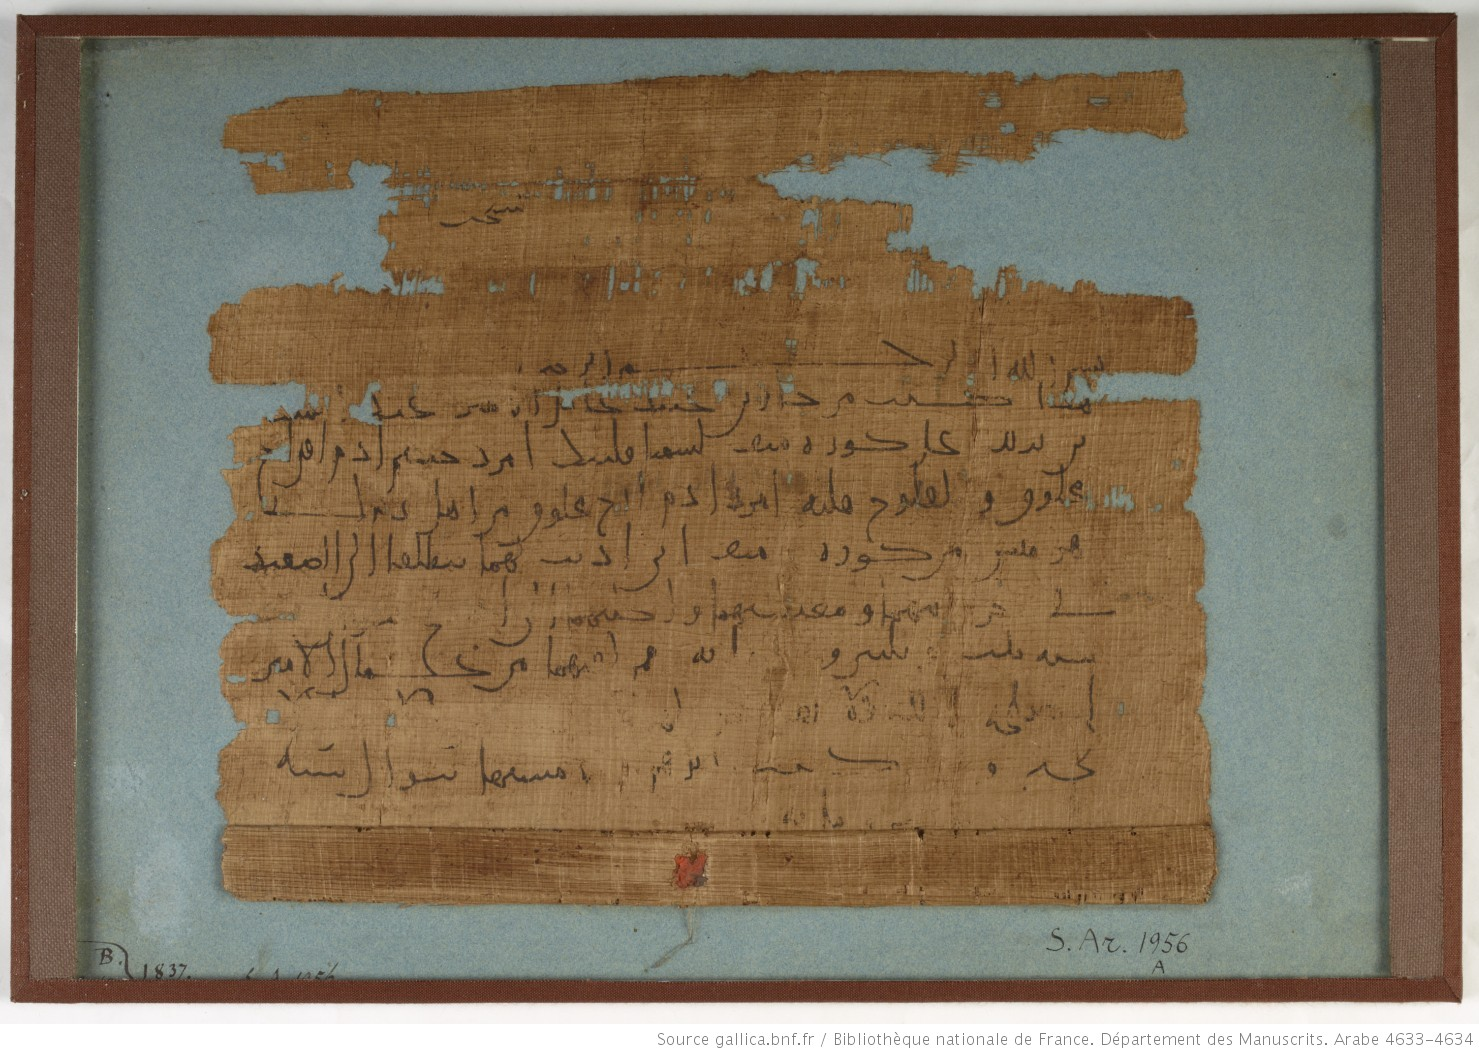
\includegraphics[width=0.68\textwidth]{images/4644.jpg}
	\caption{An Arabic papyrus showing both visible fibers and typical
	deterioration of the writing surface (BnF Arabe 4634).}
        \label{fig:papyrus}
\end{wrapfigure}

The second writing surface in wide\-spread use before the introduction of paper
in the Islamic world was parchment. Parchment is a carefully processed un- or
minimally tanned animal skin; fundamentally it can be procured from a variety
of animals and its production is not limited to a particular geographic area as
papyrus. Goat, calf, donkey, and gazelle skins, although these have never been
corroborated by testing, are mentioned as sources but the most common was sheep
skin~\cite[pg. 44]{blair2006islamic}. Its use in the East extends to time
memorial although no dated Arabic manuscripts from before the ninth century CE
survive~\cite[pg.33]{deroche2006islamic}. 

Parchment is manufactured by first removing the hair from the hide with a basic
solution made from lime or dates. Residual flesh and fat was then scraped from
the flesh side of the hide with a blade, before placing it in a wooden frame to
stretch and dry it. Finally, an abrassive stone was utilized to smooth the
surface and equalize the texture of the flesh and hair side and chalk was
applied to control bleeding of ink. Parchment were sometimes dyed with blue
indigo or yellow saffron; the most famous example of this practice is the Blue
\emph{Qurʼān} from the tenth century CE \cite[pg. 195-196]{gacek2009arabic}.

An important consideration for humanists and computer vision researchers alike,
is the ease with which previously used parchments could be reemployed by
washing or scraping off existing writing. Known as palimpsests, this practice
is attested both in the literature and by several surviving exemplars. There
could be considerably time between between the writing of the first and second
layer and examples of Arabic text over a lower layer written in another script
such as Greek or Syriac exist~\cite[pg. 43-46]{deroche2006islamic}. While the
practice was intended to remove the initial writing as completely as possible,
the lower layer often remains visibile to some extent. Separating the writing
and deciphering both texts is an immensely skilled task which can be aided by
costly multispectral imaging~\cite{easton2003multispectral}. Nevertheless the
problem has not gathered substantial research interest in the DIA community
with results from one of the few publications~\cite{starynska2017methods}
indicating that existing methods would require substantial improvement.
Parchment was also recycled in other ways, being employed in bookbinding and
protective covers to loose quires, similar to papyrus \emph{protokollon}~\cite[pg. 46]{deroche2006islamic}.

Paper was invented in China in 105 CE by the Han courtier Cai Lun. The
traditional account of its introduction to the Islamic world attributes it to a
Muslim victory in July 751 CE on the river Talas in modern-day Kazakhstan.
Chinese papermakers were supposedly taken prisoner after the battle and
dispatched to set up paper mills in Samarqand. Although the actual details of
the story can be disputed, there are etymological hints that the knowledge of
papermaking was received through Central Asia~\cite[pg. 45]{blair2006islamic}.
Paper, significantly less costly than the alternatives, rapidly displaced
papyrus and parchment as the writing surface of choice. Paper mills were
established in Baghdad by 794 CE with its use in the administration of the
Abbasid Caliphate mandated in 808 CE. By the ninth century CE its production
had spread to Egypt, by the tenth century to the Maghreb, and by the twelfth
century to Damascus and Spain~\cite[pg. 51]{deroche2006islamic}.

Apart from economical reasons paper had other benefits: it absorbes ink so
writing could not easily be erased~\cite[pg. 45]{blair2006islamic}, it is less
brittle than papyrus with a more uniform coloration, and can be easily tinted
and decorated.

The availability of an inexpensive writing material in the ninth century
produced a flurry of literary activity in subjects from theology to the natural
sciences. Books were soon copied on paper. Quranic manuscripts remained the
purview of parchment until the late tenth century CE and continued to be used
in the Maghreb and West Africa until the fourteenth century CE.

Description of papermaking in the Islamic world are sparse and unclear. In
general, a suspension of cellulose fibers is drained through a screen and
dried, resulting in a fiber mat called paper. The source of the fibers can vary
considerably: they can either be liberated from virgin plant material through a
combination of heat, beating, and chemical means such as fermentation or acids,
or originate from waste material such as rags, old ropes, etc. They are then
suspended in water to soak and collected and drained in a mold. The dried fiber
mat is called paper. An account from what is now Tunisia describes making paper
from raw flax on a floating screen. Analysis of extant specimens on the other
hand shows that waste materials, such as rags from cotton and linen or ropes,
were primarily used. Before use paper has to be sized with a mixture of
starches and egg white and burnished to prevent the ink from bleeding
excessively~\cite[pg. 44-45]{bloompaper}.

\begin{figure}[h!tp]
        \centering
	\begin{subfigure}[t]{0.3\textwidth}
		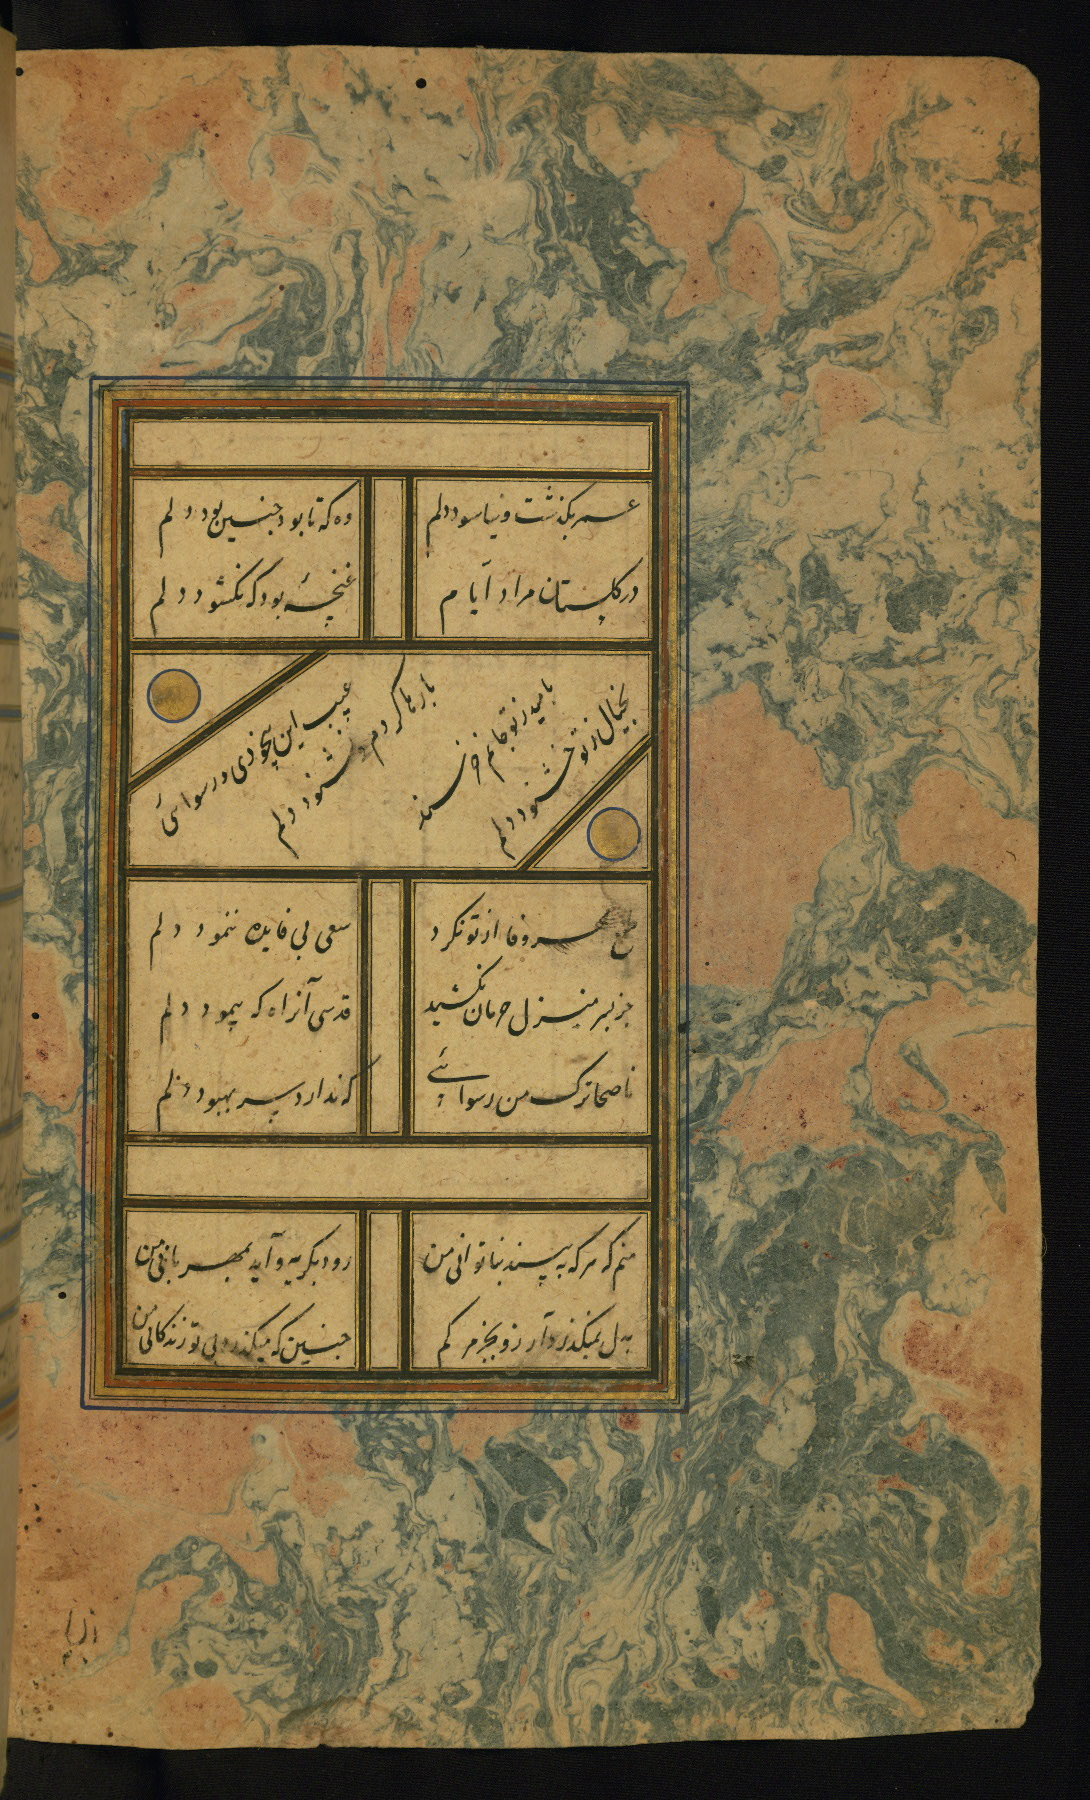
\includegraphics[width=\textwidth]{images/W654_000010_sap.jpg}
		\caption{Example of marbled paper (Walter W.654, fol. 1b)}
                \label{fig:ara_marble}
        \end{subfigure}
	\hfill
	\begin{subfigure}[t]{.3\textwidth}
                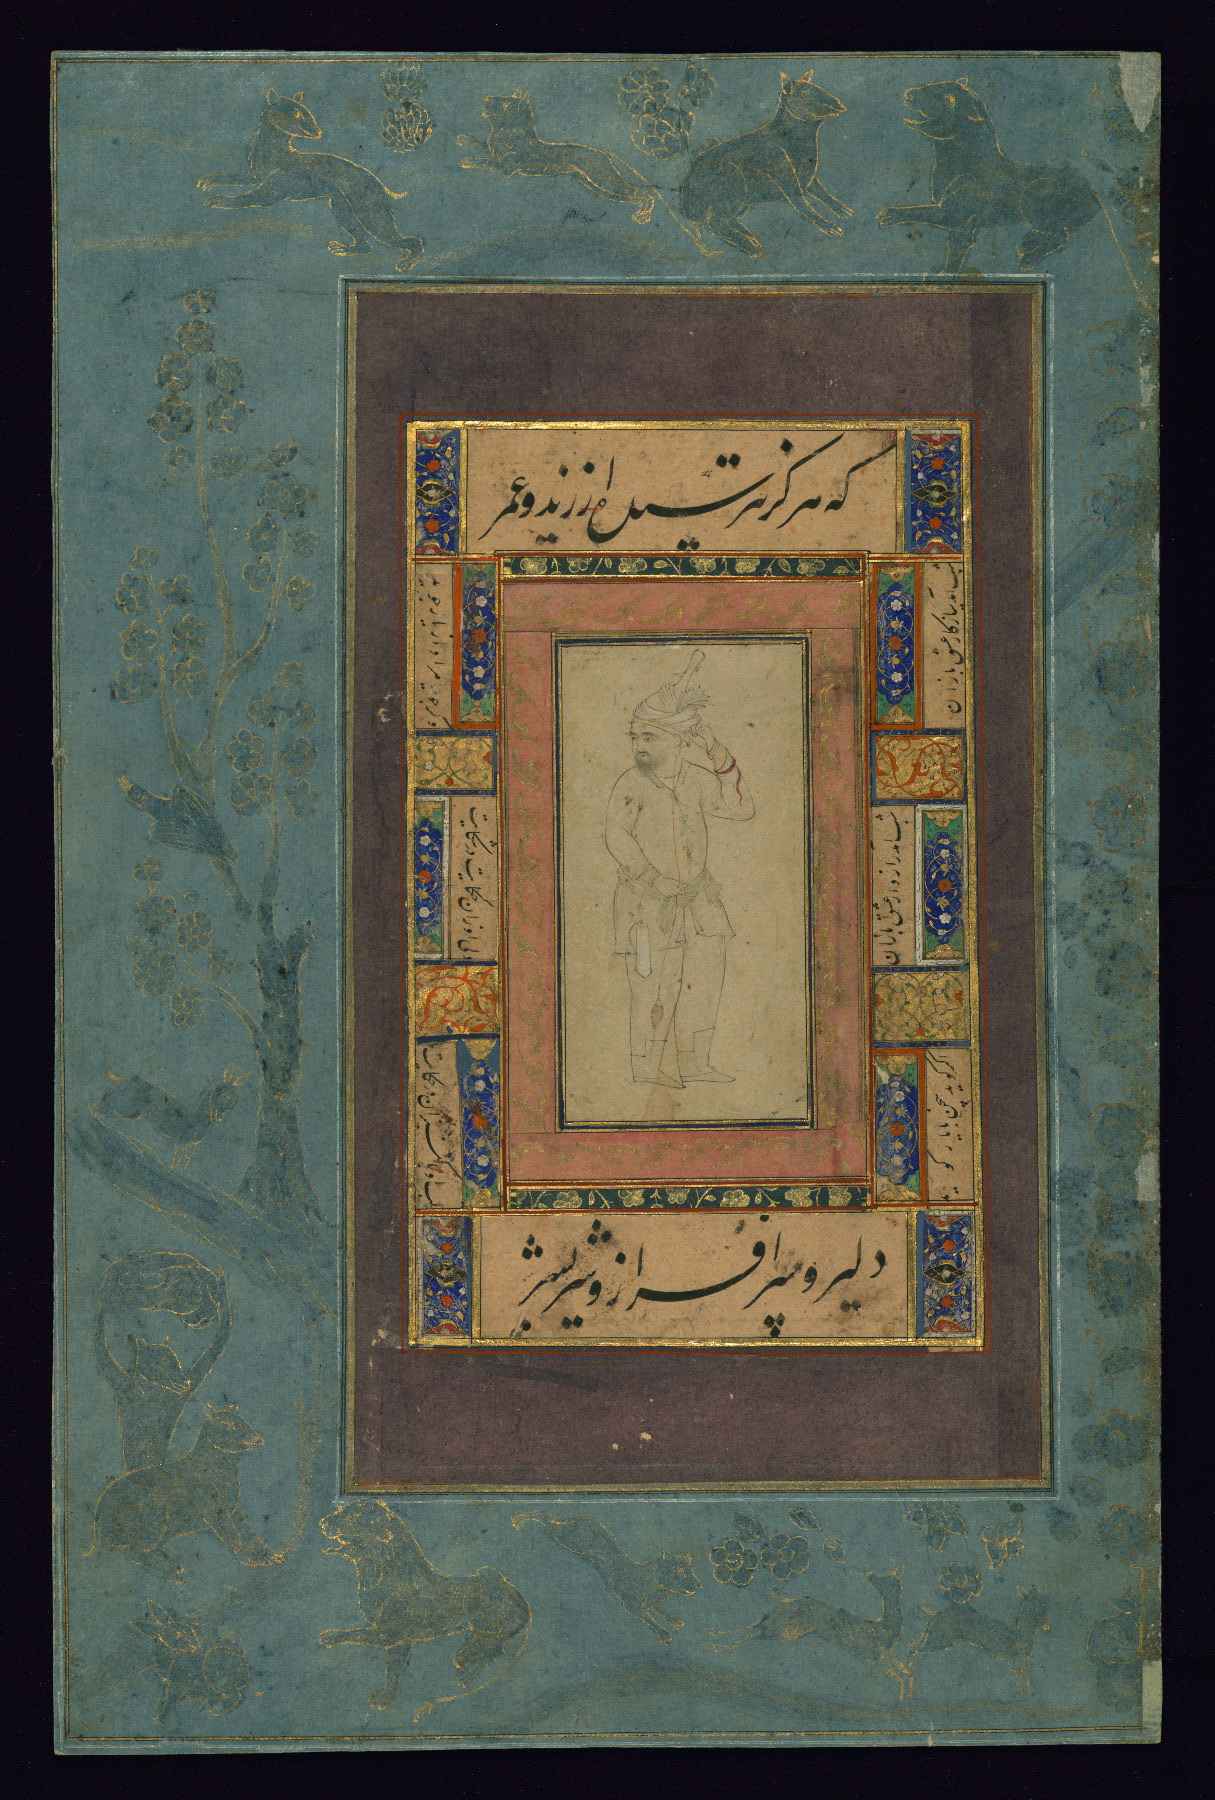
\includegraphics[width=\textwidth]{images/W746_000001_sap.jpg}
		\caption{A page with an outer border made of blue-tinted paper and an inner rose-tinted paper (Walters W.746).}
                \label{fig:ara_blue}
        \end{subfigure}
	\hfill
	\begin{subfigure}[t]{.3\columnwidth}
                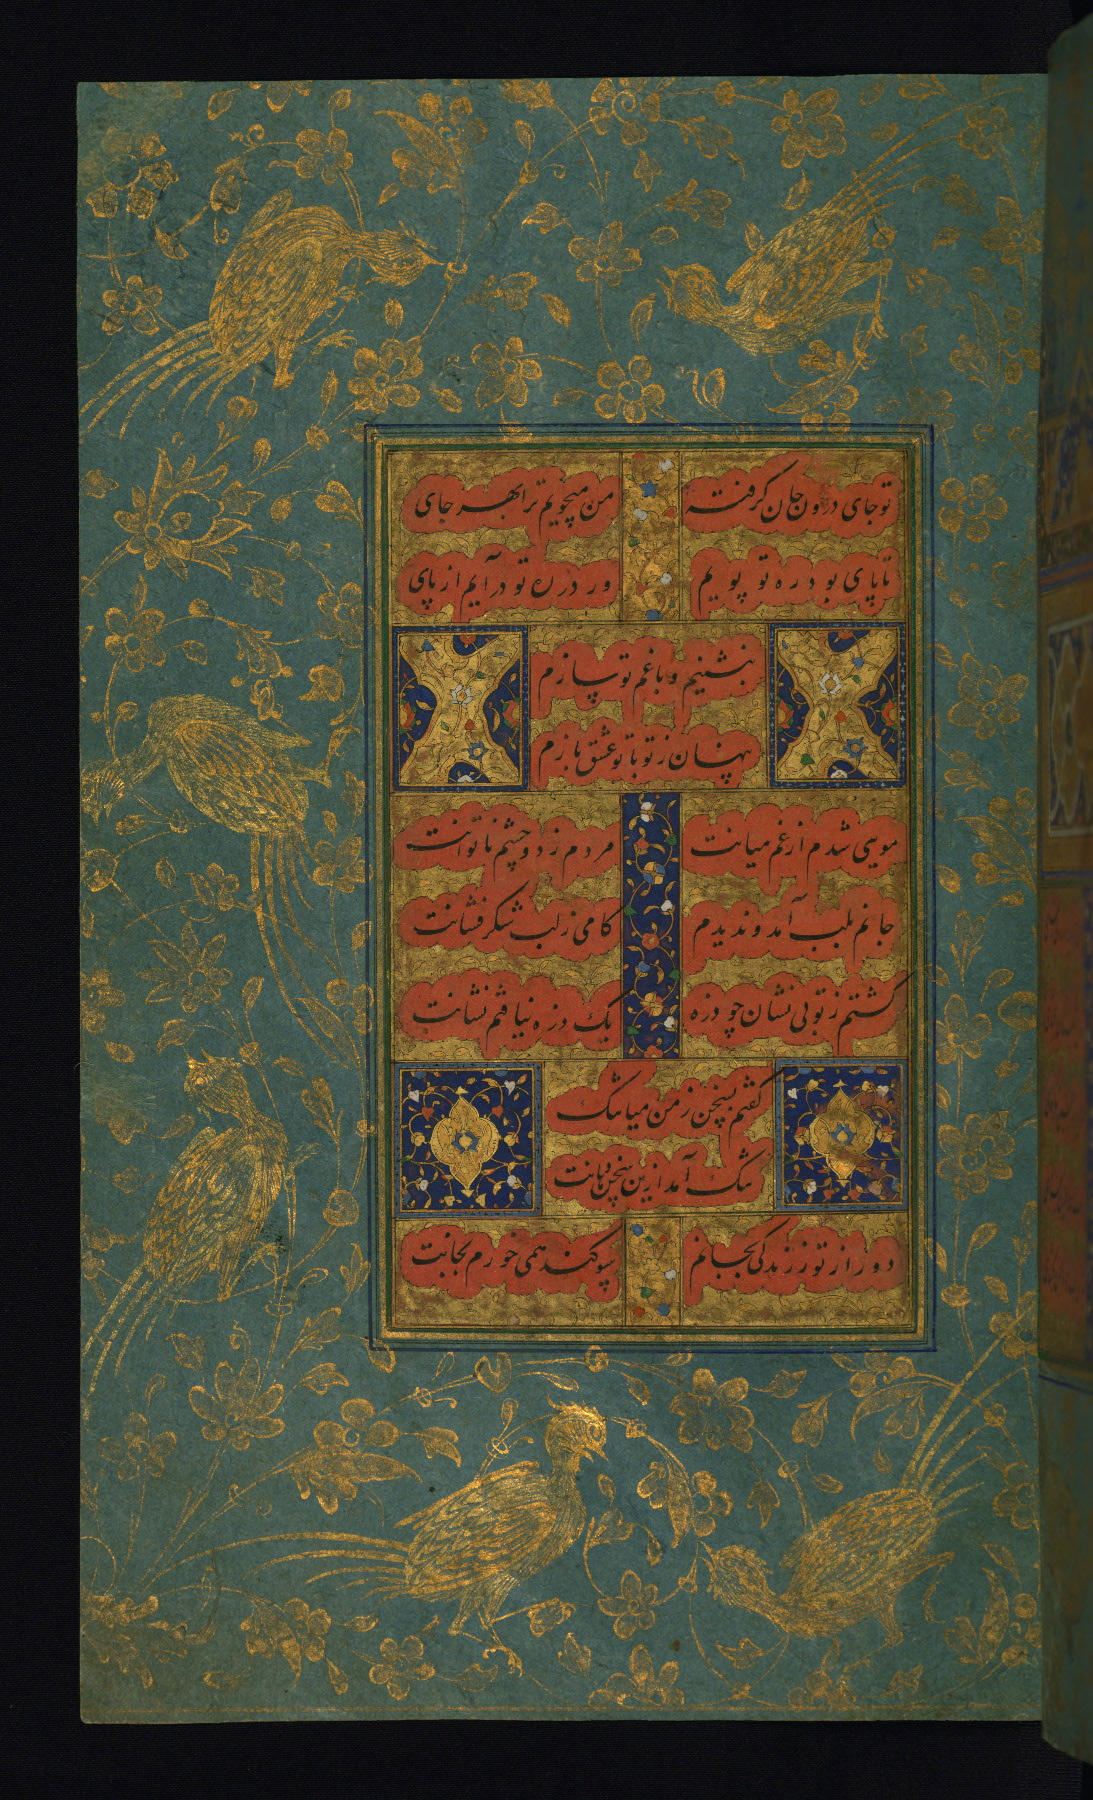
\includegraphics[width=\textwidth]{images/W651_000009_sap.jpg}
		\caption{Illumination in gold on blue-tinted border with text written on orange-tinted paper (Walters W.651, fol. 2a).}
                \label{fig:ara_orange}
        \end{subfigure}
        \caption{Decorated papers}
\end{figure}


A particularly impressive practice that often presents a challenge to modern
DIA methods are specially prepared papers used for many fine manuscripts.
Pre-modern papers retained the color of the source of the fibers, a fact that
was used in European manufacture to produce colored papers, most often various
hues of brown, but could also be tinted or dyed (figure~\ref{fig:ara_blue}).
The preference for tinted papers was probably initially fueled by colored
imports from China but Iranian artists started developing techniques to make
colored, gold-decorated, and marbled papers by the thirteenth century CE.
Popular colors were red or orange, and Persian treatises of the time list a
plethora of recipes to obtain these colors. Gold-sprinkled paper
(figure~\ref{fig:ara_orange}) was utilized throughout the Eastern Islamic lands
by the late fifteenth century CE with even more elaborate gold painting
incorporating arabesques coming into fashion from the sixteenth century onward
at the Safavid, Mughal, and Uzbek courts. Such gold-decorated papers were
mainly used in scrapbook albums of calligraphy and paintings to unify the
disparate contents into a single book. 

Other techniques rising in popularity after the fifteenth century CE are
marbled papers (figure~\ref{fig:ara_marble}) and paper cuts. While the marbling
produced by slipping a sheet of paper over a bath of carefully swirled colorant
cause the same issues to DIA methods as other decorated margins, paper cuts are
likely more complicated.  Cut-out calligraphy, either collage, i.e. placing
cut-out letters on a contrasting background, or decoupage, i.e. mount a sheet
with cut out letters above a differently colored one, allows larger variation
in coloration than purely ink-based writing. Artists were often skilled in more
than one of these techniques and they are often employed together. Works such
as a collection of forty hadith for the Ottoman prince Mehmed in 1540 CE,
contain text in both \emph{taw'qī} and \emph{nastaʼlīq} script, pasted in gold,
white, or light blue on deep-rose or olive grounds. The margins on some pages
are kept plain, others gold-sprinkled, others again marbled~\cite[pg.
52-56]{blair2006islamic}. The sheer variety of printing even contained in a
single manuscript are sure to challenge any DIA system.

\subsection{Writing Instruments and Inks}

The Arabic script is traditionally written with a reed pen whose front had been
trimmed with a special pen knife to create a nib. Depending on the desired
width of the script the nib was slit one or more times at its end. Multiple nib
cuts existed. While straight and oblique cuts changed the thickness of strokes
at certain angles, the association of cut angles and scripts seems to have been
largely a matter of scribal preference~\cite[pg. 42]{gacek2009arabic}.

Brushes were primarily used in the process of decoration, such as paintings in
the margins or gilding. Chinese muslims developed the rounded, flowing
\emph{ṣīnī} script in the fourteenth century CE to adapt Arabic writing to the
instruments and conventions of Chinese calligraphy, even going so far as to
change the directionality of the writing to top-to-bottom in some
cases~\cite[pg. 29-30]{ghoname2012sini}.

Of more pertinence to the application of document image analysis than the
writing instruments are the inks and pigments employed in writing. Three kinds
of black or brown inks were commonly used: carbon-based inks, so-called mixed
inks, and iron gall inks, although compound inks were common in the medieval
period~\cite[pg. 62-63]{blair2006islamic}. All were known in the area of the
later Islamic lands since antiquity. Carbon inks are attested as far back as
the second millenium BCE in Egypt while the first recipes for mixed inks dating
to the third century BCE and iron gall inks being in use by the fifth century
CE~\cite{christiansen2017manufacture}.

Carbon inks, more commonly known as India inks, are composed of fine soot or
finely ground charcoal mixed with some kind of binder, such as oil, gums, or
shellac. For portability they were often carried as a solid stick that is
ground and mixed with water before use. The main source for carbon used in inks
in the muslim world was from the combustion of vegetable matter such as rice,
olives, and chick-peas or various oils. The most common binders were gum arabic
and honey~\cite[pg. 133]{gacek2009arabic}. Inks prepared in this manner adheres
only superficially to the writing surface, can easily be washed off with water
and smudge easily when kept in humid conditions or peels off over time. An
improvement are the so-called mixed inks that are made of carbon inks to which
copper, lead, or iron salts were added. These were intended to increase
adherence to the paper and functioned as drying agents. Iron gall inks do not
contain any carbon and functions by oxidation of the ink once applied to the
paper which forms an insoluble ferric tannate pigment. It is prepared by mixing
tannic acid extracted from gallnuts, vitriol (ferric sulfate), and a binder
such as gum arabic. In contrast to the previous two inks it penetrates the
writing surface and is indelible \cite{christiansen2017manufacture}. Their
major drawback is their acidic nature and fading over time. Manuscripts written
in iron gall ink are often damaged by acid burns to the point of being
illegible to human readers and computer vision methods alike~\cite[pg.
145]{gacek2009arabic}

Colored inks were utilized by scribes and calligraphers as accent colors for
rubrics, vocalization, and other decoration. Red, green, and yellow were most
widely employed. Although the pigments used in the manufacture of these inks
have not been systematically studied, cochineal, vermillion, and red lead
contained in red, lapis lazuli and azurite in blue, and verdigris in green
inks. There is also substantial regional differentation with different pigment
and color use between the east and the west~\cite[pg. 63]{blair2006islamic}.
Coloration of this kind is largely unproblematic to modern DIA methods,
although pipelines employing binarization will encounter substantial
degradation as the most commonplace binarization algorithms perform quite
poorly on mixed-color texts. Of more universal troublesomeness are metallic
inks, such as in figure~\ref{fig:ara_muhaqqaq}, not for their inherent
illegibility but the low contrast exhibited by scanned documents. Both fine
metals such as gold and silver and copper were used in at least two different
ways: liquid inks, made of metal flakes suspended in a binder~\cite[pg.
225-227]{raggetti2019inks}, and dispersing powdered flakes onto glue which were
subsequently burnished and ringed with other colors. Writing produced with the
latter technique is often liable to degradation as disintegration of the glue
has caused flakes to fall off~\cite[pg. 63]{blair2006islamic}.

\section{Styles}

A large number of formal and informal calligraphic styles have been devised
over the centuries. While informal styles naturally evade uniform
classification, the formal styles can be grouped into ones that are recognized
throughout the Muslim world, such as \emph{naskh}, and ones that are largely
limited to a certain geographical region or only used to write specific
languages, such as the North African and Iberian \emph{maghribi} or the Persian
\emph{nastaʼlīq}  

Arabic styles can be defined by elements such as~\cite[pg. 242-243]{gacek2009arabic}:

\begin{description}
	\item[Line of writing] whether all words sit completely on the
			       baseline, descend onto it as in
			       \emph{nastaʼlīq}, curve upwards toward the end,
			       or are slanted.
	\item[Ascender and descenders] vertical, slanted or curved
	\item[Nib width] especially in relation to script size.
	\item[Shading] i.e. contrast between thin and thick strokes.
	\item[Vocalization] Some scripts require a different pen for vocalization.
	\item[Ligatures] The presence of unauthorized connections between letters.
	\item[Contractions] The presence of assimilated (omitted) letter forms.
	\item[Characteristic letterforms] such as straight, wavy, or slanted \emph{ʾalif}
\end{description}

The two earliest styles that emerged in the seventh century CE are
\emph{ḥijāzī} (figure~\ref{fig:ara_hijazi}) and kufic
(figure~\ref{fig:ara_kufic}. Both are somewhat confusingly named after early
Islamic intellectual centers (Hijaz and the city Kufa in southern Iraq) and a
variety of alternative terms such as Early Abbasid have been proposed. As
canonicalization was fairly low the terms do not refer singular hands but to
families of styles that were used mainly to transcribe copies of the
\emph{qurʼān}. One taxonomy divides them into six and four groups for the kufic
and \emph{ḥijāzī} family respectively. Either is notably more angular than
later round styles.  Hijazi being in use from 650 CE it was surplanted by kufic
by the beginning of the eighth century CE. While elaborate, highly decorated
manuscripts in the kufic style survive, the number of surviving Hijazi
fragments is very low and their appearance is utilitarian \cite[pg. 98,
124]{gacek2009arabic}.

\begin{figure}[h!tp]
        \centering
        \begin{subfigure}{\textwidth}
		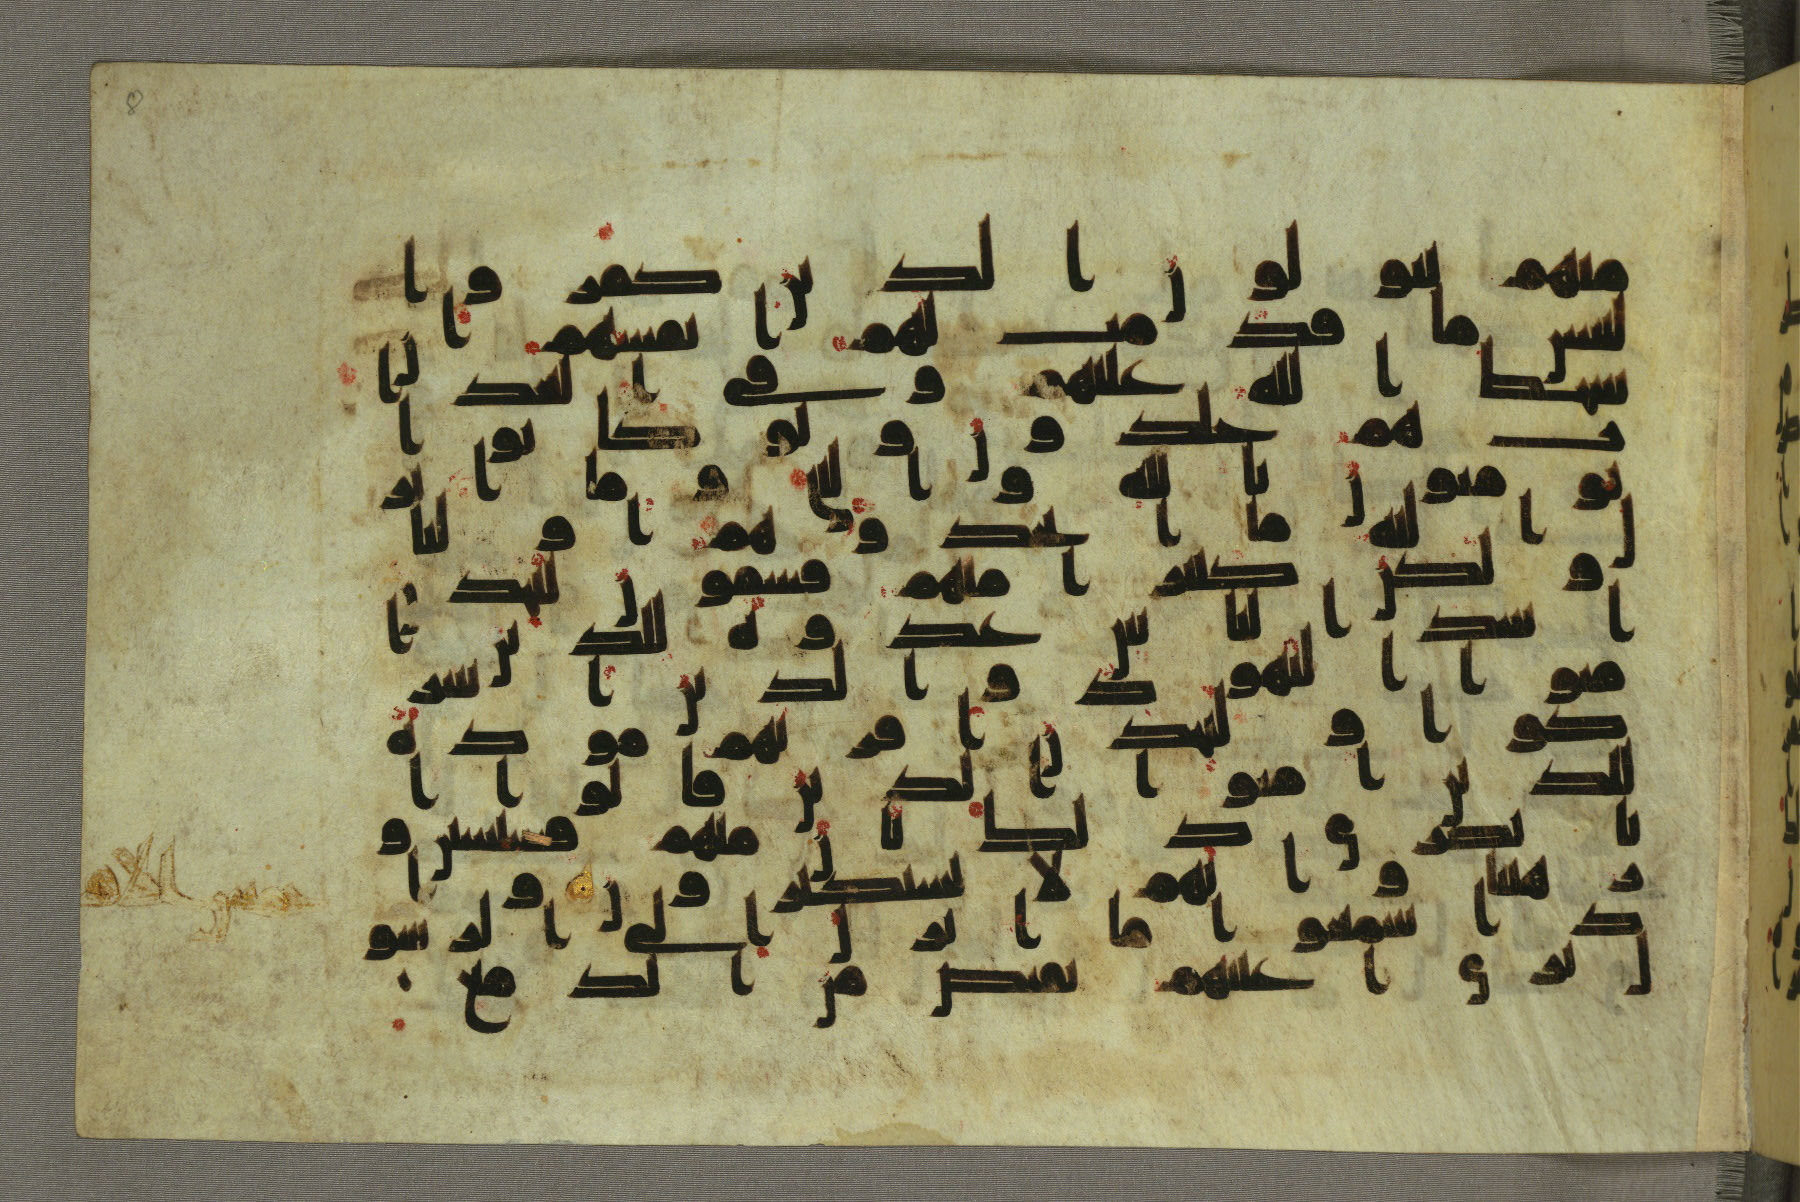
\includegraphics[width=\textwidth]{images/W552_000024_sap.jpg}
		\caption{Ninth century CE \emph{qurʼān} in Kufic or Early Abbasid script (Walters W.552, fol. 8a)}
                \label{fig:ara_kufic}
        \end{subfigure}
        \vskip\baselineskip
	\begin{subfigure}[t]{.48\textwidth}
                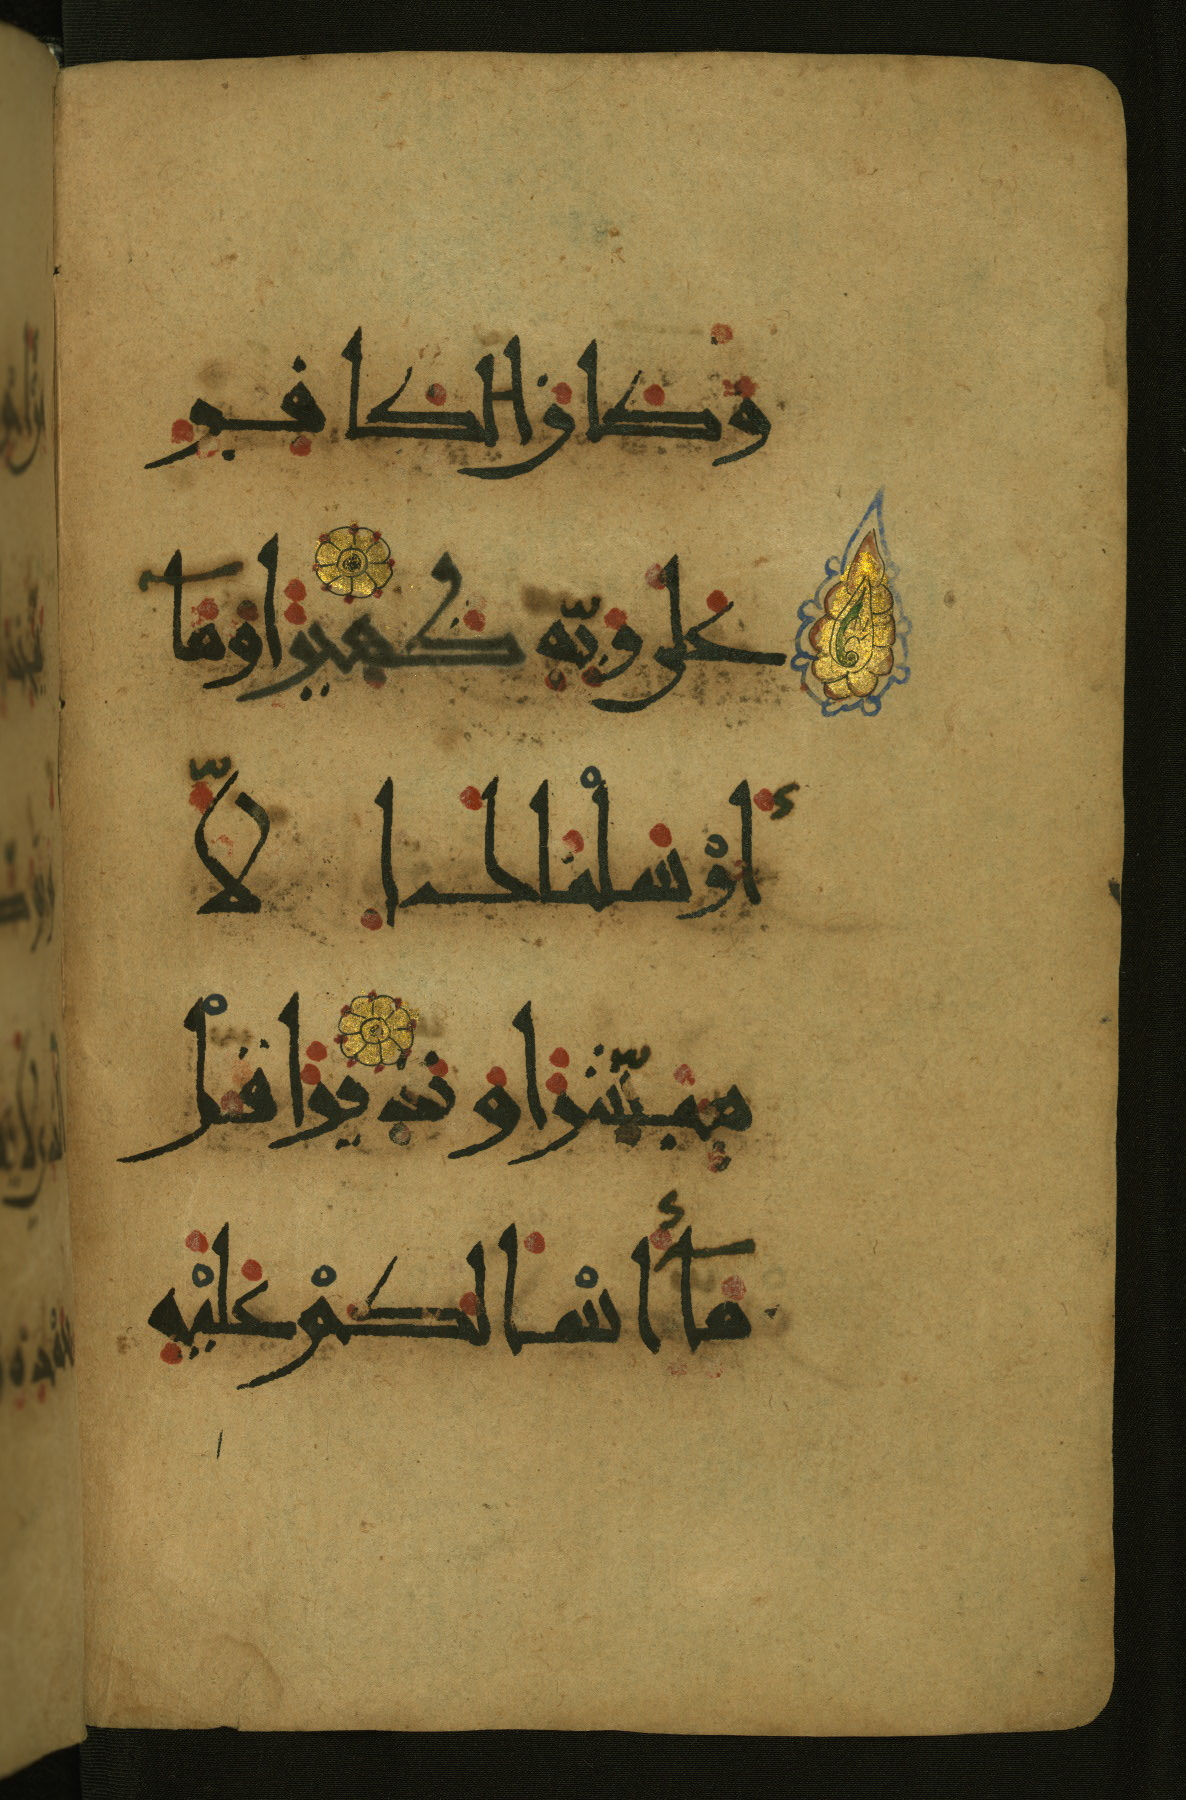
\includegraphics[width=\textwidth]{images/W555_000024_sap.jpg}
		\caption{Twelfth century CE \emph{qurʼān} in broken cursive or New Abbasid script (Walters W.555, fol. 10b)}
                \label{fig:ara_broken}
        \end{subfigure}
	\hfill
	\begin{subfigure}[t]{.48\columnwidth}
                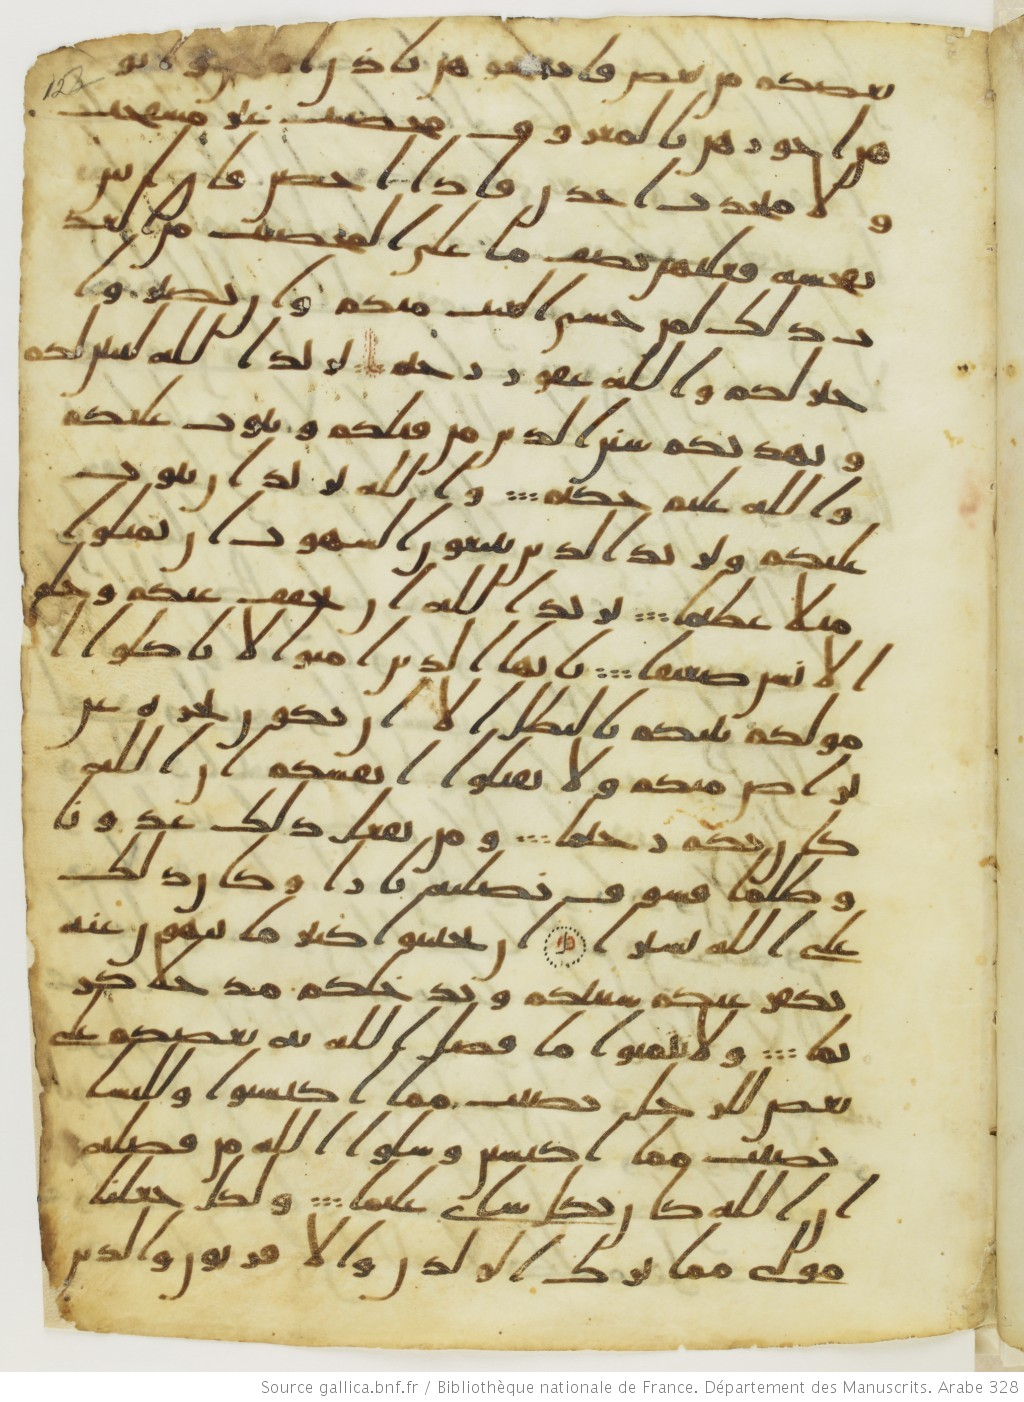
\includegraphics[width=\textwidth]{images/Coran__btv1b8415207g_31.jpeg}
		\caption{Seventh century CE \emph{qurʼān} in \emph{ḥijāzī} script (BnF Arabe 328, fol. 12r)}
                \label{fig:ara_hijazi}
        \end{subfigure}
        \caption{Early Arabic styles}
\end{figure}

By the tenth century CE the use of kufic in high status manuscripts began to be
replaced by a style known under a variety of names such as Eastern kufic, New
Abbasid Style, and broken cursive~\cite[pg. 144]{blair2006islamic}
(figure~\ref{fig:ara_broken}). This style was dominant into the thirteenth
century CE for copies of the \emph{qurʼān} when it was relegated to ornamental
purposes such as titles and headings. As with older styles, it represents not a
single hand but at least two different groups. The main characteristics of this
style is the marked difference between thick and thin strokes \cite[pg.
167-168]{gacek2009arabic}. From this period also dates the practice of using
long \emph{taṭwīl} elongation to mark the start of a new section of
text~\cite[pg. 165]{blair2006islamic}.

\subsection{The Six Pens}

The responsibility for the advancement of the Arabic script until the
thirteenth century CE is traditionally assigned to three great calligraphers:
Ibn Muqlah (d. 940), Ibn al-Bawwab (d. 1022), and Yaqut (d. 1298). The
fundamental development of the period between the tenth and thirteenth century
is the system of proportioned scripts and the canonicalization of the various
rounded styles under this system. Ibn Muqla is attributed with developing the
first proportioned script, \emph{al-khatt al-mansub}, that defined each
letter's dimensions in the unit of rhomboid dots, impressions left by the reed
pen on the writing surface, with \emph{alif} spanning a circle circumscribing
all other graphemes. While this system is most likely only a thirteenth century
CE attempt at reconstructing the hand of the famous calligrapher, as none of
his works survived, Ibn al-Bawwab is credited with canonicalizing the round
chancery scripts in use at the time using this system~\cite[pg. 158-160,
213]{blair2006islamic}. Finally, the popularization of the six proportional
styles known as the \emph{Six Pens} as the dominant scripts in the East falls
during the lifetime of Yaqut~\cite[pg. 251]{gacek2009arabic}.

These six styles are usually paired in three sets of one display (majuscule)
and one text (minuscule) script:

\begin{itemize}
	\item \emph{thuluth} with \emph{naskh}
	\item \emph{muḥaqqaq} with \emph{rayḥān}
	\item \emph{tawqīʿ} and \emph{riqāʿ}
\end{itemize}

\begin{figure}[h!tp]
        \centering
        \begin{subfigure}{\textwidth}
		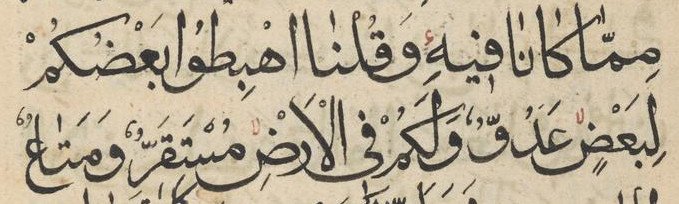
\includegraphics[width=\textwidth]{images/6940_0010_web.jpg}
		\caption{Two lines written in \emph{thuluth} from an undated copy of the \emph{qurʼān} (Columbia University, MS Or 234, fol. 4v).}
                \label{fig:ara_thuluth}
        \end{subfigure}
        \vskip\baselineskip
        \begin{subfigure}{\textwidth}
		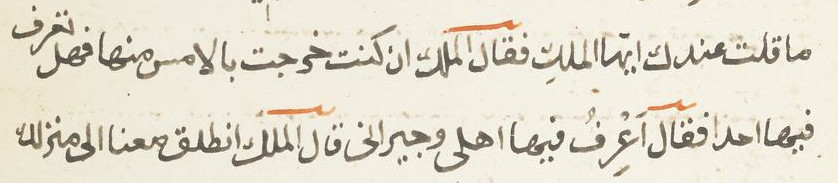
\includegraphics[width=\textwidth]{images/9224_0009_web.jpg}
		\caption{Two lines written in \emph{naskh} from an undated book of quranic stories (Free Library of Philadelphia, Lewis O 170, fol. 5r).}
                \label{fig:ara_naskh}
        \end{subfigure}
        \vskip\baselineskip
        \begin{subfigure}{\textwidth}
		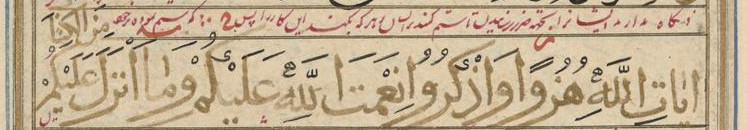
\includegraphics[width=\textwidth]{images/6937_0054_web.jpg}
		\caption{Central line in \emph{muḥaqqaq} in gold of a bilingual
		Arabic and Persian copy of the \emph{qurʼān}. The red line
		above is part of the interlinear Persian translation in
		\emph{nastaʼlīq} (Columbia University, Ms Or 222, 23r).}
                \label{fig:ara_muhaqqaq}
        \end{subfigure}
        \vskip\baselineskip
        \begin{subfigure}{\textwidth}
		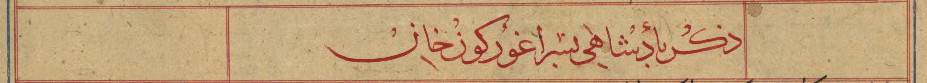
\includegraphics[width=\textwidth]{images/W676_000004_sap.jpg}
		\caption{Chapter heading written in  \emph{tawqīʿ} script from a fifteenth century CE Timurid history (Walters W.676, fol. Bb).}
                \label{fig:ara_tawqi}
        \end{subfigure}
        \vskip\baselineskip
        \begin{subfigure}{\textwidth}
		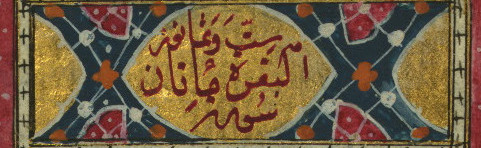
\includegraphics[width=\textwidth]{images/W567_000005_sap.jpg}
		\caption{Heading in \emph{riqāʿ} script of a nineteenth century CE \emph{qurʼān} copy (Walters W.567, fol. 2a).}
                \label{fig:ara_riqa}
        \end{subfigure}
	\caption{Samples of five of the Six Pens}
\end{figure}


\emph{Thuluth} (figure~\ref{fig:ara_thuluth}) is an ancient chancery script
although its exact features are unknown prior to its reform to the proportioned
script system in the eleventh century CE. Its most notable properties are
descenders which fall far below the baseline and curve upwards again for
certain letters, hairlines, and many contracted letterforms. As a display
script its letter are large but horizontally compact. In administrative use it
was utilized for important documents while in codices it was used mainly for
titles and chapter headings~\cite[pg. 275]{gacek2009arabic}.

\emph{Naskh} (figure~\ref{fig:ara_naskh})  is the most widely used bookhand of
the Islamic East. It is a serifless script without unauthorized connections
between letters, long ascenders, and short descenders. Some Persian and Ottoman
variations of the script exist. It is the basis for most modern Arabic
typefaces intended for use in prose~\cite[pg. 162-163]{gacek2009arabic}.

\emph{Muḥaqqaq} (figure~\ref{fig:ara_muhaqqaq}) is one of the ancient scripts
originally devised before the proportioned scripts system. It is rectilinear,
i.e. only a small proportion of the penstrokes are curved or curvilinear. It is
a seriffed script with vocalization performed with a different pen, often in a
different color. While grouped as the display script to \emph{rayḥān} it also
became a bookhand for copies of the \emph{qurʼān} by the thirteenth century
CE~\cite[pg. 160-161]{gacek2009arabic}.

\emph{Rayḥān} is the smaller counterpart to \emph{muḥaqqaq}. The letter forms
were identical except for their size, the inclusion of serifs, and the
execution of vocalization with the same pen as the letters~\cite[pg.
308]{EncyclopediaofArabicLanguageandLinguisticsVolume3}.

\emph{Tawqīʿ} (figure~\ref{fig:ara_tawqi}) is a smaller diplay variant of the
\emph{thuluth} chancery script being written with even more hairlines. Like
\emph{thuluth} it was rarely used as a bookhand~\cite[pg.
264-264]{gacek2009arabic}.

\emph{Riqāʿ} (figure~\ref{fig:ara_riqa}) is the smaller version of the
\emph{tawqīʿ} script. It is optionally seriffed with slightly rightward
inclined \emph{alif}. In Iran the differences between it and \emph{tawqīʿ} were
minor with one publication using the terms synonymously~\cite[pg.
224]{gacek2009arabic}.

\subsection{Regional Styles}

At the same time a number of regional scripts developed. In the Maghreb, Muslim
Spain, and West Africa a number of scripts emerged that were later summarized
under the name \emph{maghribī} (figure~\ref{fig:ara_maghribi}). These
non-proportioned  hands are distinctive but no detailled paeleographical
analysis has been done to date and there exist a number of sub-types. One
shared feature is the use of a rounded nib resulting in even thickness of
strokes~\cite[pg. 147-148]{gacek2009arabic}.  The earliest manuscripts in these
styles date to the mid-tenth century CE with the earliest surviving
\emph{qurʼān} copy dated to 1008 CE but little change occured
afterwards~\cite[pg. 566]{blair2006islamic}.

In Iran, at the same time as Yaqut was refining the Six Pens, two new styles of
hanging script called \emph{taʿlīq} (figure~\ref{fig:ara_taliq}) and
\emph{nastaʼlīq} (figure~\ref{fig:ara_nastaliq}) emerged. These were more
suitable for writing languages such as Persian and Turkish that differ from
Arabic in their proportion of straight and curved letters. As such they were
never popular in the Arabic speaking world but \emph{nastaʼlīq} ended up as the
style of choice for a number of other states such as Ottoman Turkey and Mughal
India. The highly stylized \emph{taʿlīq} script with its curvilinear elements,
extraneous loops, and connected letter was a typical style for official
decrees, diplomatic correspondence, sometimes poetry, but almost never codices,
from the tenth century CE. The stereotypical \emph{taʿlīq} document contains
widely spaced lines with dramatic upward curving at the end of the line. A
variant broken \emph{taʿlīq} replaced it from the fourteenth century CE in
administrative use~\cite[pg. 270-273]{blair2006islamic}.

\begin{figure}[h!tp]
        \centering
	\begin{subfigure}[t]{.48\columnwidth}
                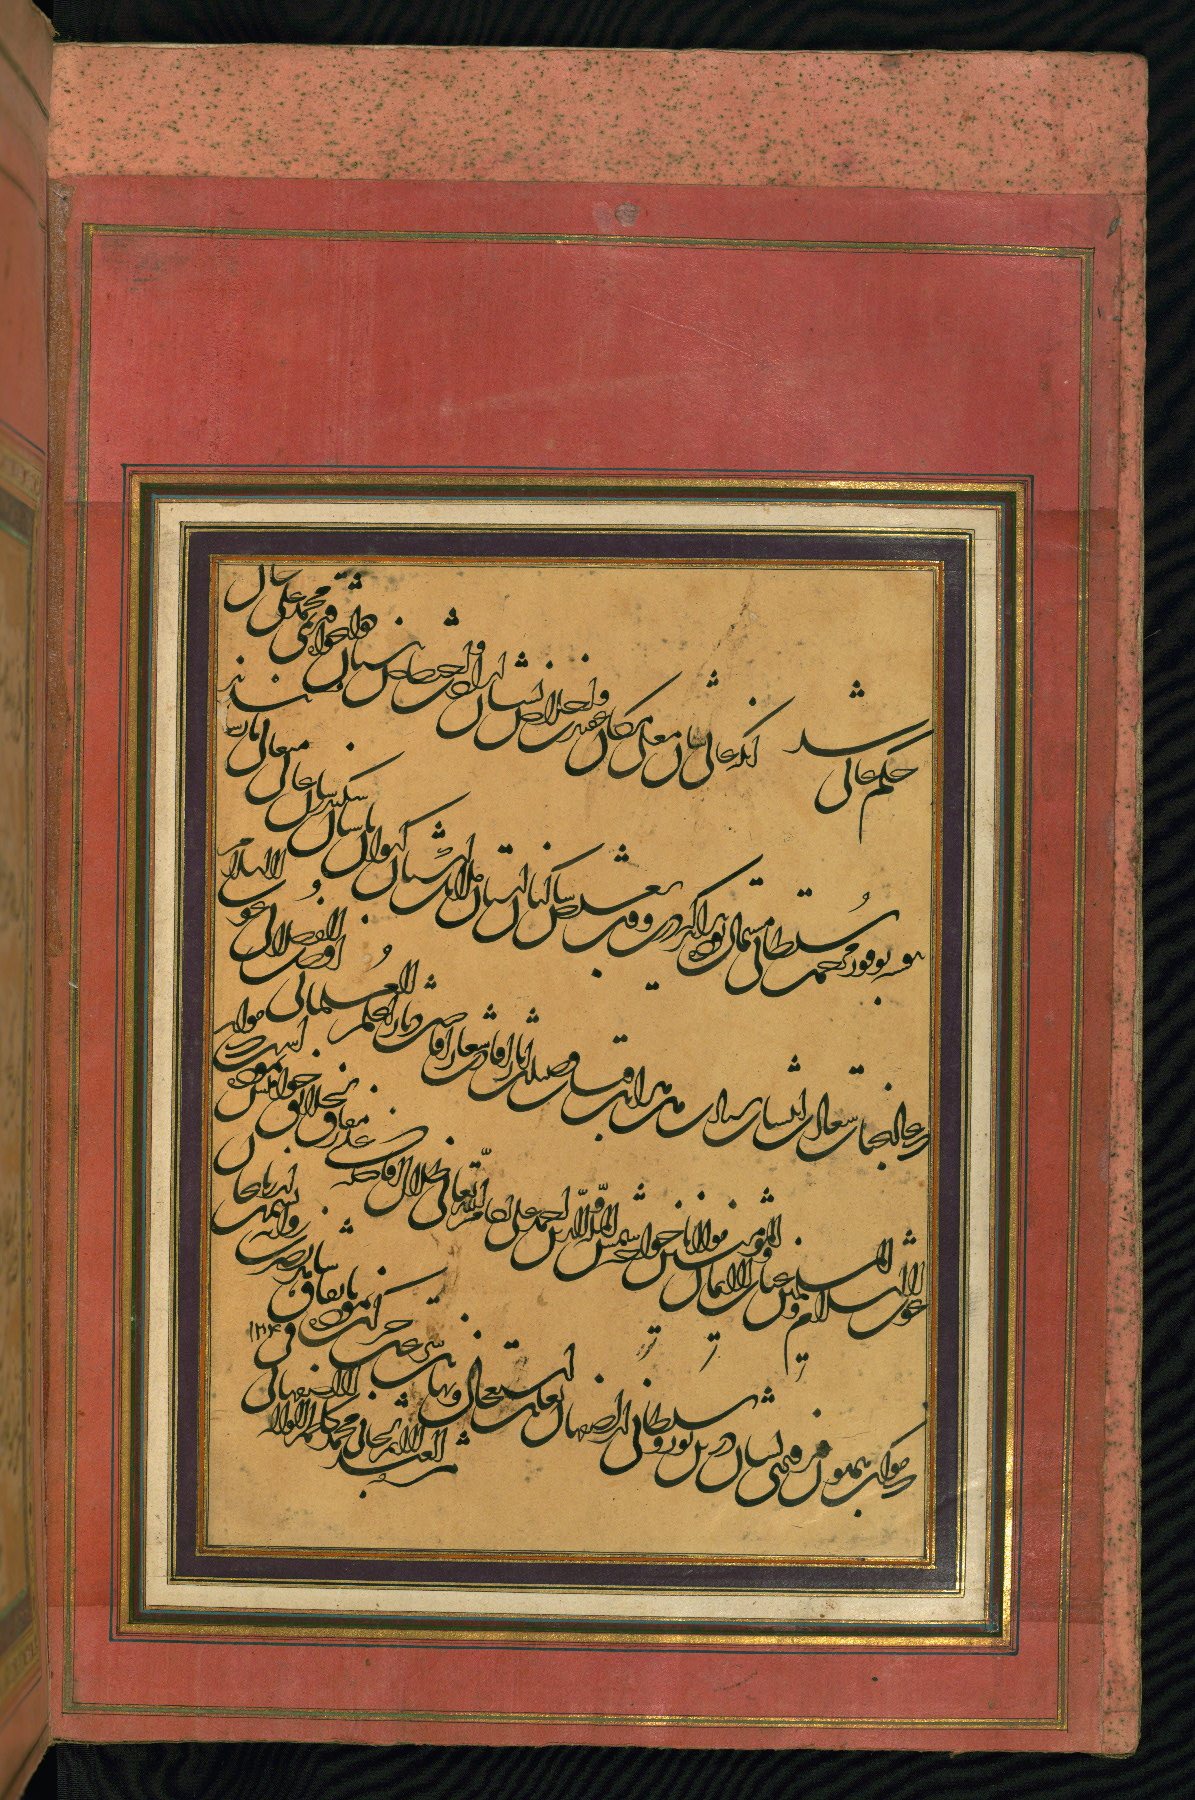
\includegraphics[width=\textwidth]{images/W670_000040_sap.jpg}
		\caption{Page from a Persian nineteenth century CE album of calligraphic samples written in \emph{taʼlīq} (Walters W.670, fol. 19b)}
                \label{fig:ara_taliq}
        \end{subfigure}
	\hfill
	\begin{subfigure}[t]{.48\columnwidth}
                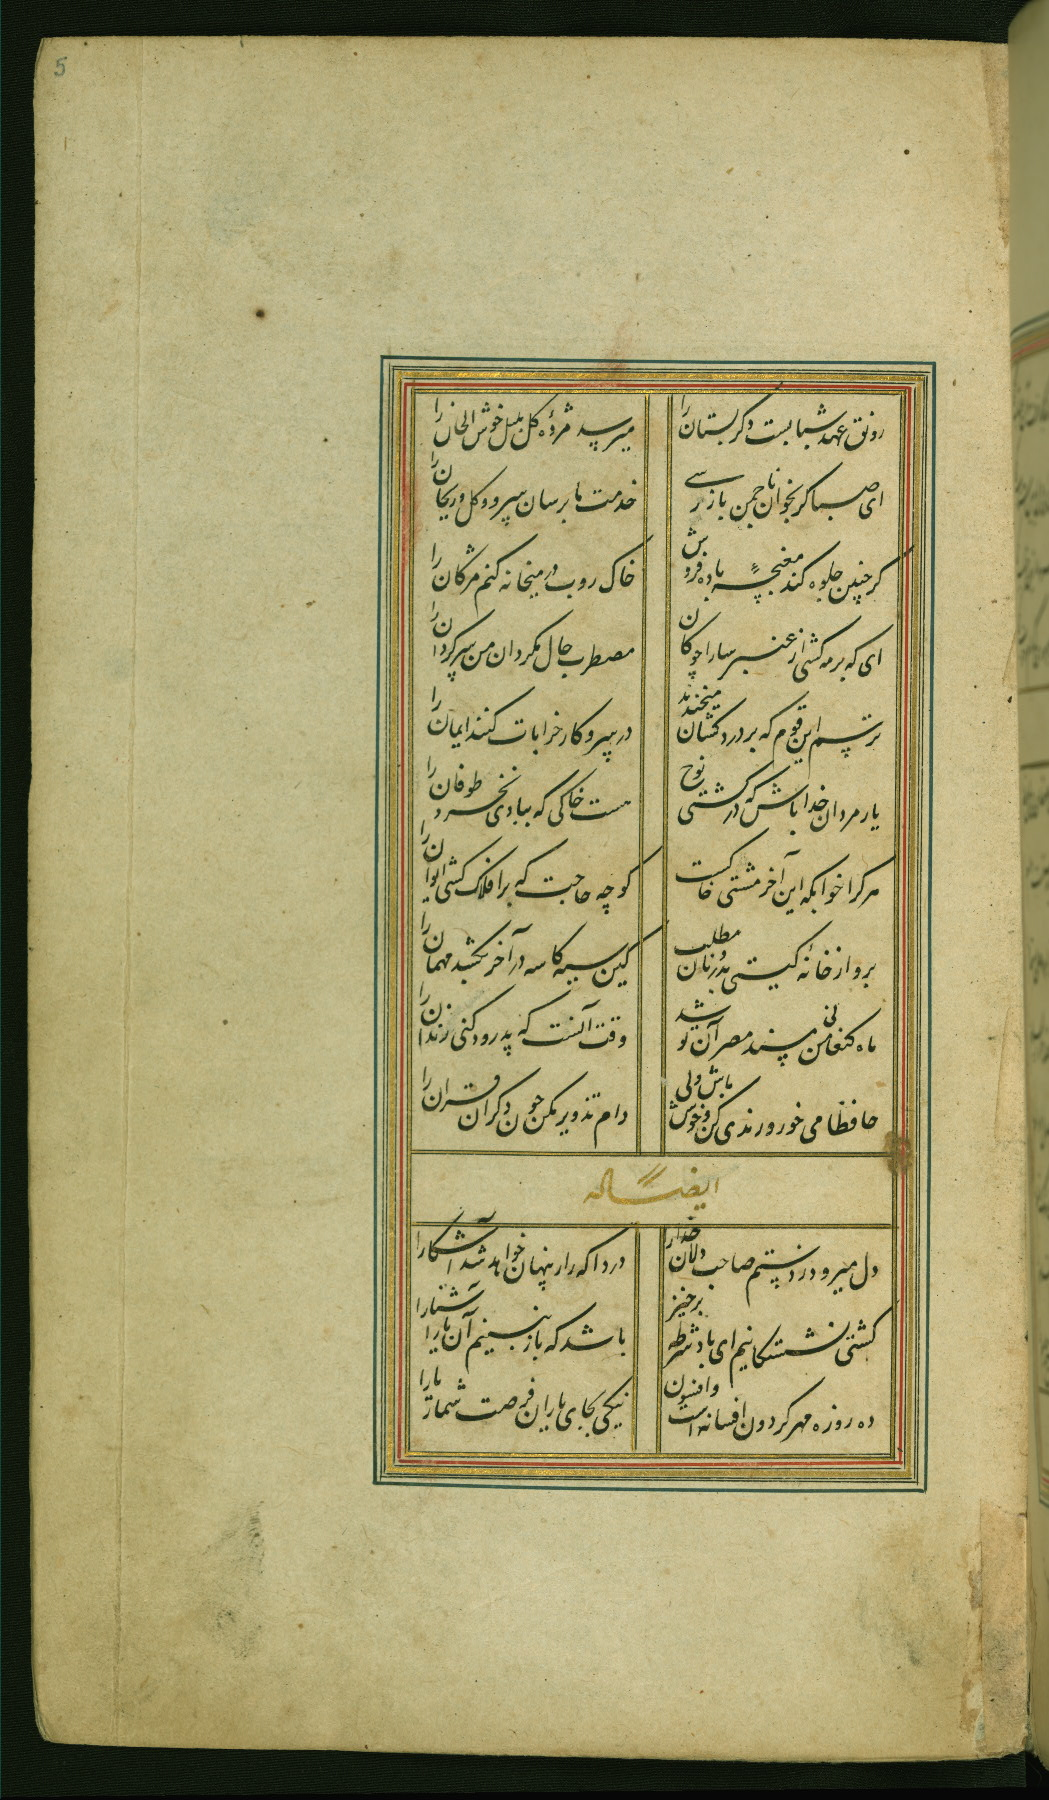
\includegraphics[width=\textwidth]{images/W631_000014_sap.jpg}
		\caption{1539 CE page from a collection of poems written in \emph{nastaʼlīq} (Walters W.631, fol. 5a)}
                \label{fig:ara_nastaliq}
        \end{subfigure}
        \vskip\baselineskip
	\begin{subfigure}[t]{.48\textwidth}
		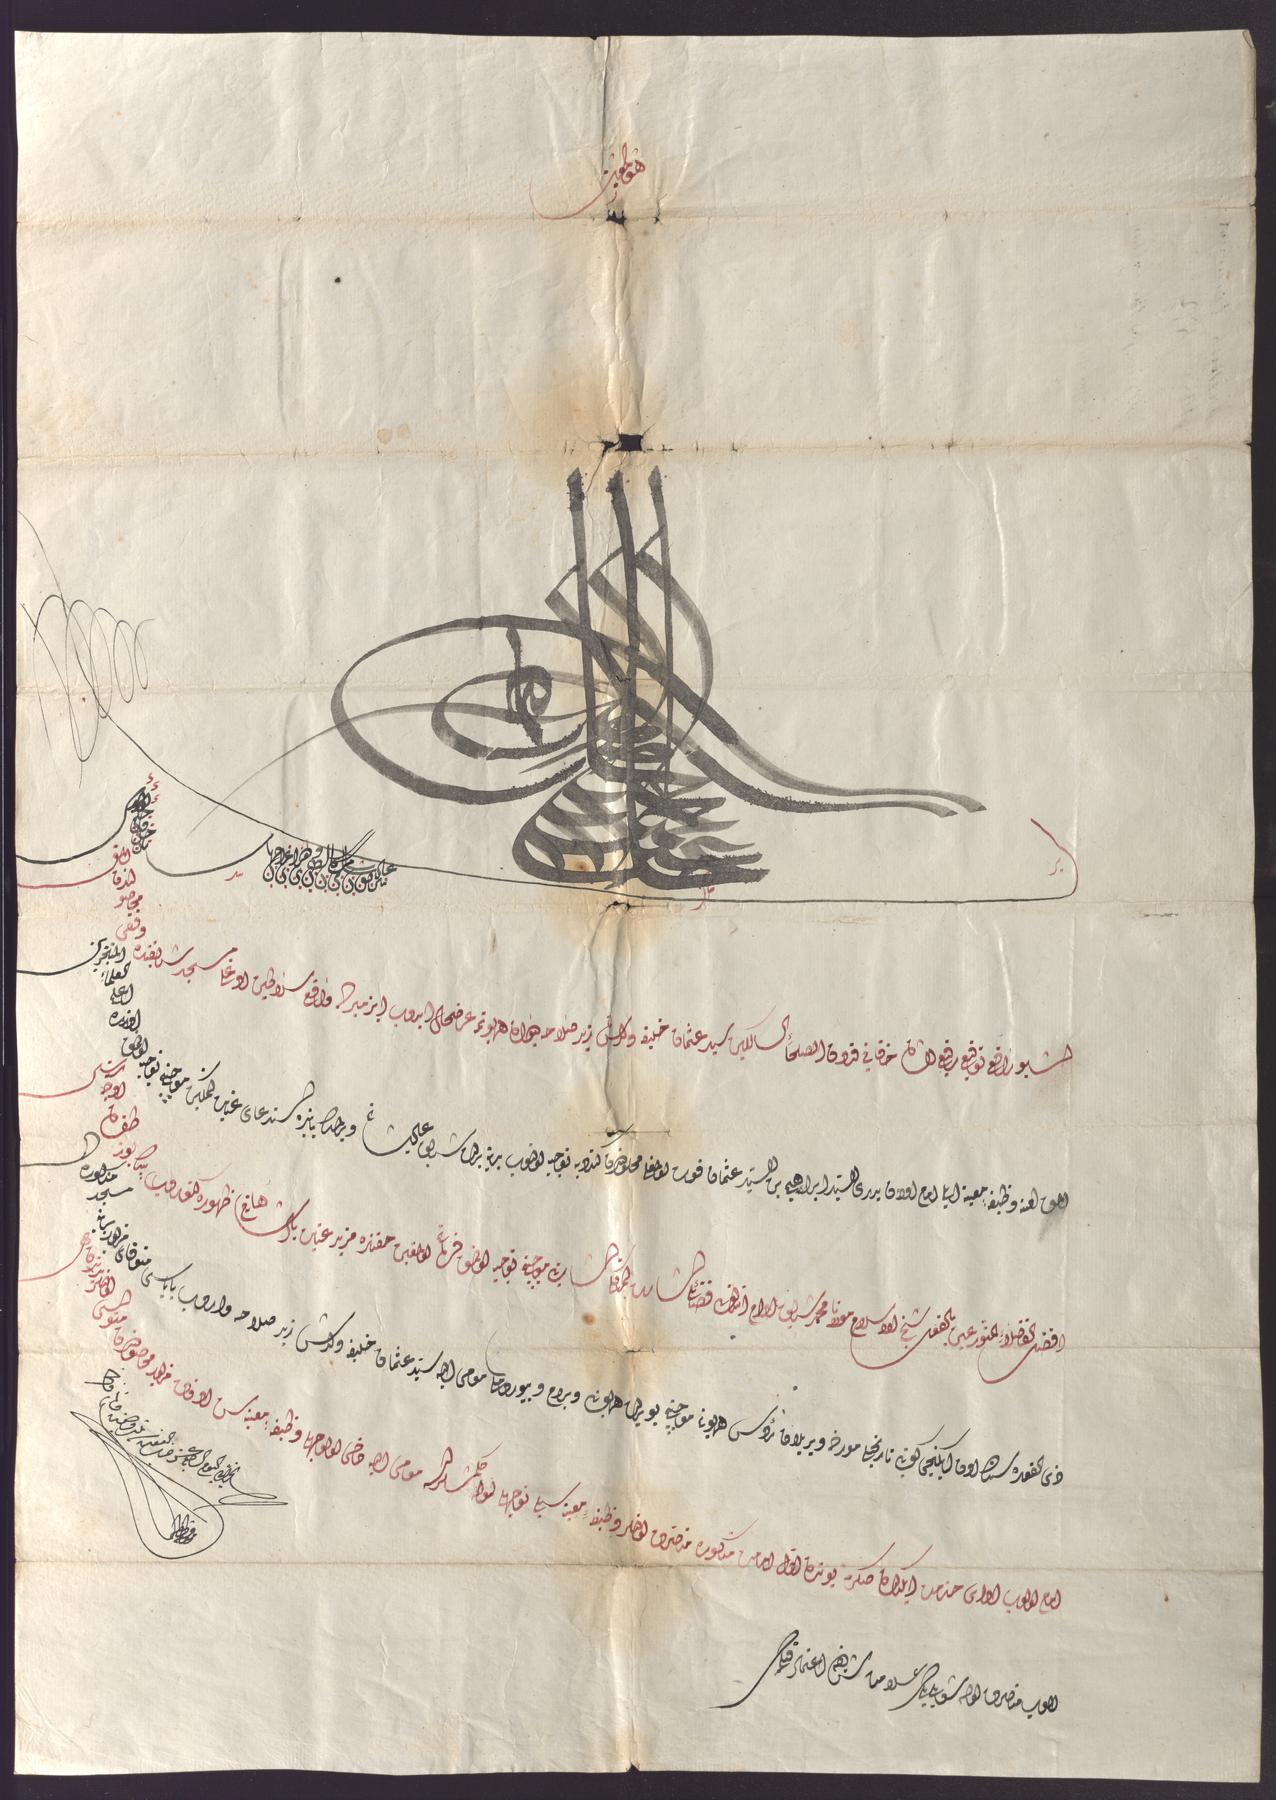
\includegraphics[width=\textwidth]{images/9676_0002_web.jpg}
		\caption{1779 CE Ottoman firman \emph{diwānī} script (American Philosophical Society Ms. Coll. 200, fol. 2)}
                \label{fig:ara_diwani}
        \end{subfigure}
	\hfill
	\begin{subfigure}[t]{.48\textwidth}
                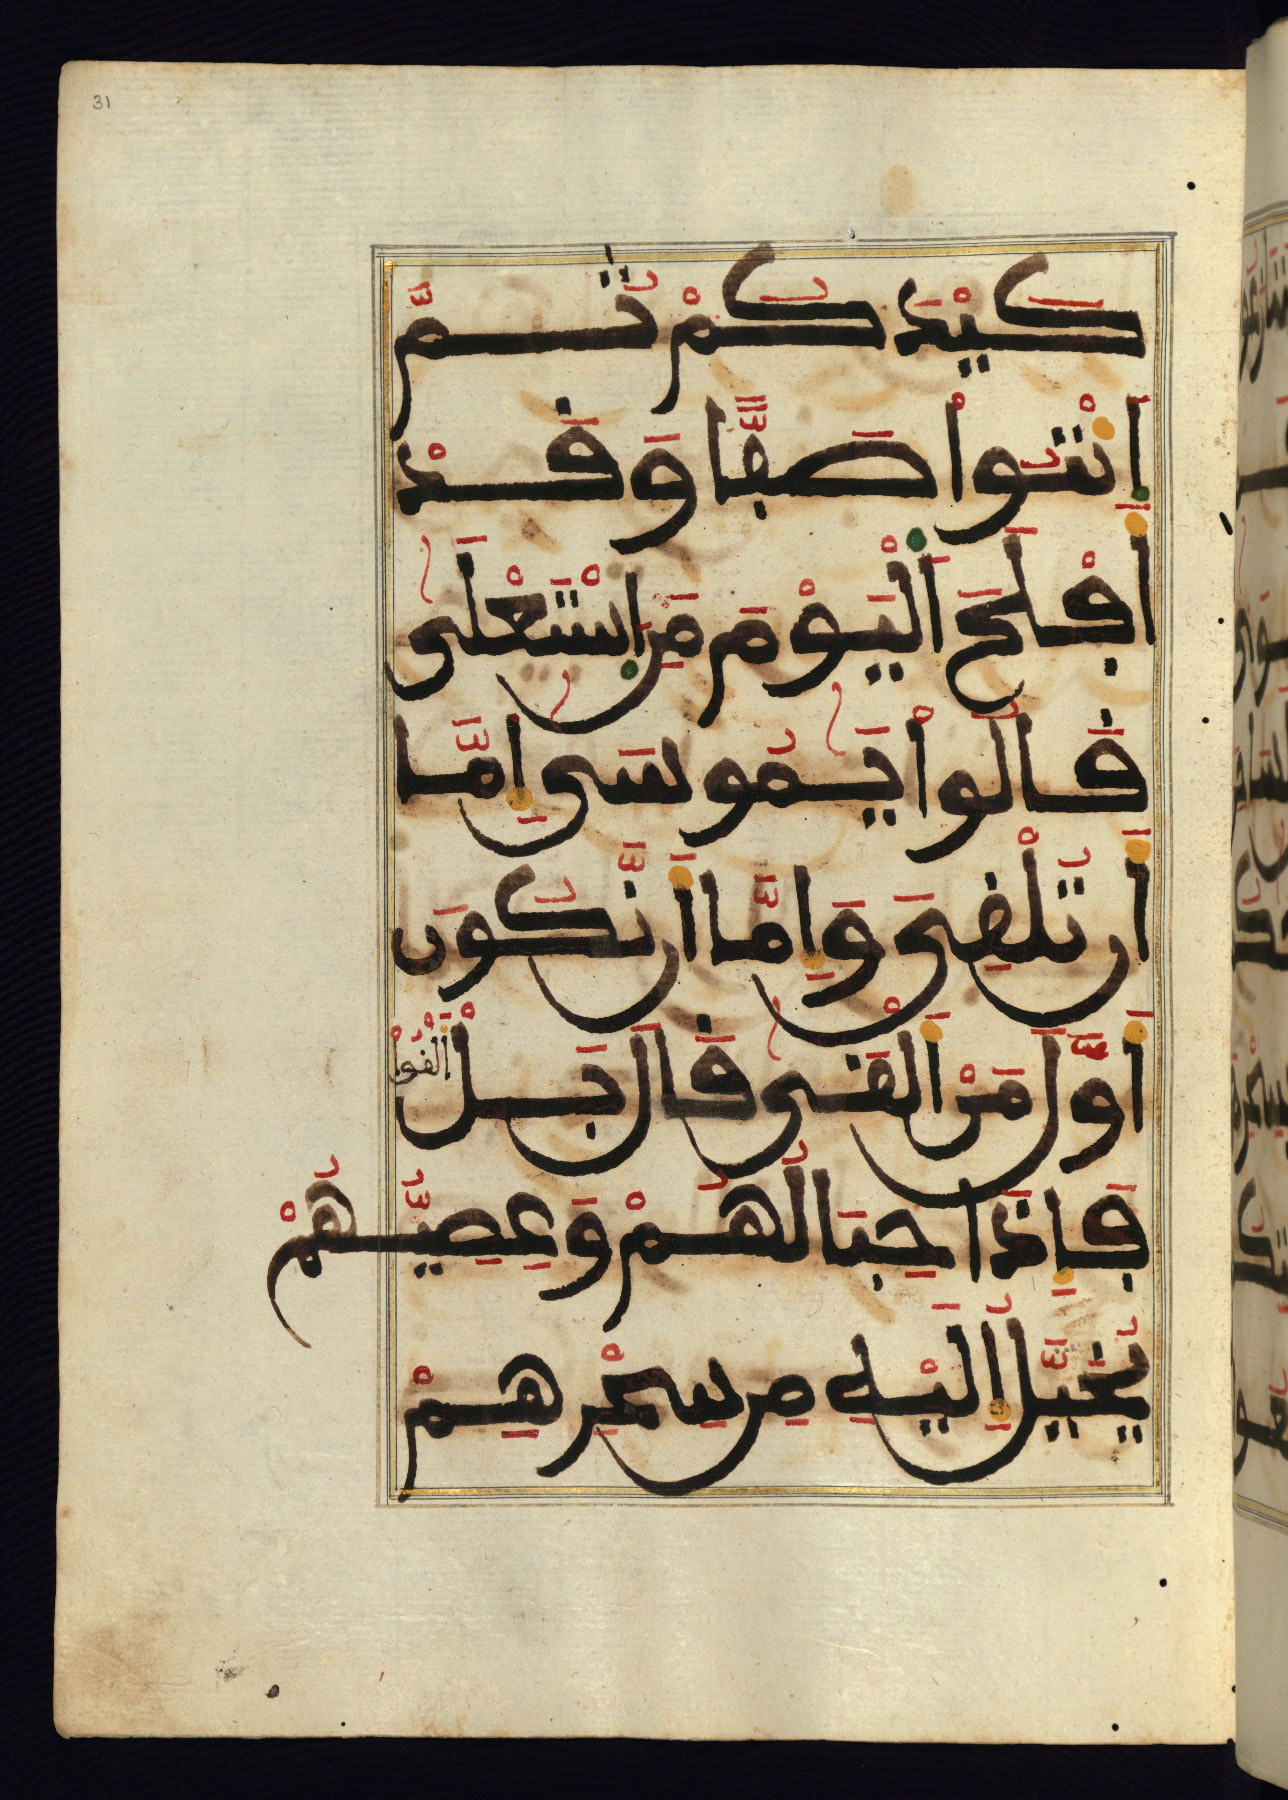
\includegraphics[width=\textwidth]{images/W568_000064_sap.jpg}
		\caption{Nineteenth century CE \emph{qurʼān} in large \emph{maghribī} script (Walters W.568, fol. 31a)}
                \label{fig:ara_maghribi}
        \end{subfigure}
        \caption{Example of regional styles}
\end{figure}


The second major Persian style, \emph{nastaʼlīq}, became the epitome of Persian
literature. At first reserved for poetry, it took over the place of
\emph{naskh} for prose by the fifteenth century as well. It is characterized by
individual words descending onto a common baseline, greatly elongated
horizontal lines, and the aforementioned heaping of the last stroke~\cite[pg.
166-167]{gacek2009arabic}. While the aforementioned styles, depending on the
preservation of the document, the desired generalization, and accuracy, are not
inherently troublesome for a modern OCR engine, the sophistication displayed by
the most decorated \emph{nastaʼlīq} epics and calligraphic specimens are highly
challenging. Calligraphers of the time were interested in variety and visual
excitement, arranging verses on the diagonal, changing direction between
successive verses, alternating red, blue, orange, and green inks for headings,
and adding lavish illumination and scrollwork. The writing was being subsumed
by decoration~\cite[pg. 436]{blair2006islamic}. 

Both round scripts, primarily \emph{naskh} and \emph{thuluth}, and Persian
hanging scripts were common in the Ottoman Empire with their relative
proportion in text production varying over the centuries\footnote{\cite[chapter
XI]{blair2006islamic} elaborates the cycles of popularity between round and
hanging scripts.} In the fifteenth century CE imperial scribes began to develop
the \emph{taʿlīq} script into the highly stylized \emph{diwānī}
(figure~\ref{fig:ara_diwani}) chancery style with its unauthorized connections
between letters and curved baselines.

\section{Printing}

While the main focus of this dissertation is the question of handwritten text
recognition, printing of the Arabic script deserves some consideration,
especially as its development and diffusion is directly linked to the practice
of calligraphy. Printing is the mechanical reproduction of text and images.
Since the printing system developed by Johannes Gutenberg around 1450 the term
has been near-synonymous with movable type printing where reverse images of
each grapheme including punctuation marks and decorations are cast in metal as
individual elements, the type. Types are arranged to form larger units, most
often whole lines, which are subsequently assembled into a matrix for a whole
page. The matrix is placed in a printing press, inked, brought into contact
with the material to be printed, usually paper, and the process is repeated as
desired. Nevertheless other kinds of printing, such as Egyptian and
Mesopotamian cylinder seals or Chinese woodblock printing, have existed for
thousands of years before Gutenberg's invention. 

In contrast to movable type printing, block printing employs a unitary matrix
carved out of a single piece of wood. The production of block printed texts has
been attested throughout Islamic world since at least 900 CE, although the
practice seems to have died out by 1430. The actual extent of the use of this
technique and its exact origins are still unknown and the low number of
block-printed documents in archives and the lack of archeological evidence for
matrices and printing equipment leave the topic mostly shrouded in obscurity.
The only preserved documents with any frequency are amulets and charms
containing quranic passages printed on paper in a wide array of styles,
generally following equivalent calligraphic practices of their handwritten
counterparts\footnote{A survey of the current state of scholarship is found in
\cite{schaefer2006enigmatic}}. As these documents have largely escaped the
scholarly interest, there are up to now no specific methods developed by the
DIA community to treat them.

Movable type printing arrived in the Islamic world at the end of the fifteenth
century CE with printing presses being set up in Constantinople and other
cities of the Ottoman Empire. While these were operating in Islamic lands, they
were run by the Jewish minority and did not produce books in Arabic script.
Evidence for the popularly held notion that the Ottoman Sultan Bayezid II
prohibited movable type printing outright, restricted it to certain scripts, or
minorities of the empire in 1485 CE is contradictory and slim
\cite{schwartz2017did} but in any case printing of the Arabic script in the
Islamic world was first performed in the workshop established by imperial
printer Ibrahim Muteferrika in 1727 CE. This does not mean that no Arabic books
were printed at all but these were exclusively imports, mostly from workshops
in Italy. The earliest preserved print is a book of hours from 1513 CE printed
in Venice by Gregorio de Gregori~\cite{krek1979enigma}. The earliest printed
edition of the \emph{qurʼān} was produced by the brother Paganino and Alessandro
Paganini in 1537-1538 CE and was an utter commercial failure as the typeface
was odd and the text itself riddled with numberous errors~\cite[pg.
219-220]{bloompaper}. Even typefaces later cut by famed type-founders such as
Robert Granjon (1585), William Caslon (1720), Giambattista Bodoni (1759) were
simplistic and of low quality~\cite{tracy1975advances}. 

Although universally derided for their lack of grace, legibility, and
orthographical correctness later imports seem to have found more popular
acceptance as lamented by Muteferrika in a 1727 CE work on the usefulness of
printing. The secular nature of the vast majority of these imports support the
theory that religious sentiment was a principal factor hindering the adoption
of printing, although the economic interests of a substantial class of scribes
and calligraphers certainly played a role, in addition to the inherent
difficulties of creating adequate typefaces for a cursive script~\cite[pg.
605]{blair2006islamic}.

Despite this multi-faceted resistance to movable type printing, some refinement
took place. While typeface cut in the Christian world were largely modelled on
the \emph{maghrebi} style, Muteferrika introduced the more legible \emph{naskh}
style in printing which remains to this day the most popular style for printed
Arabic texts. However, creating a full Arabic font remained a truly staggering
task; the Imprimerie Nationale's twenty-four-point nineteenth century CE Arabic
typeface contained 710 different types~\cite[pg. 218]{bloompaper}. In addition,
actually setting such large typefaces required skill incomparable to the much
simpler Latin script. It has been argued that apart from social objections, the
sheer laboriousness combined with a lacking industrial base made movable type
printing uneconomical in the Islamic world \cite{auji2017neither}. Indeed, the
rise of printing presses in the nineteenth century coincides with the invention
of lithography which allowed inexpensive, accurate reproductions of handwritten
texts, missionary activity and modernization drives less subject to immediate
economic pressures \cite{turner1996dictionary}. Printers like Faris al Shidyaq,
founder of the al-Jawa'ib press in Istanbul, introduced Western-style layouts
with punctuation marks and paragraphs but were not able to resolve the
laborious typesetting process or aesthetic issues such as lacking overlap of
letters, line justification limited to baseline stroke elongation instead of
the more aesthetically pleasing letter elongation or stacking, and visible gaps
between individual types~\cite[pg. 605]{blair2006islamic}. The invention of hot
type line casting machines such as the 1911 Arabic Linotype eliminated gaps
between glyphs but the limits of the machine did not allow proper placement of
vowel marks~\cite[pg. 67]{nemeth2017arabic} and subsequent iterations
economised more and more glyph variants reducing the visual appeal of the final
product. Only the advent of software-driven phototypesetters in the
nineteen-sixties make sufficiently large type repertoires including contextual
and elongated forms economically feasable. Even though the last vestiges of the
limitations of physical type have disappeared with purely digital typesetters,
most common typefacess do not make use of these.

A closer study on the limitations of current OCR technology on modern printed
Arabic texts follows in the next chapter.

\section{Basic requirements for Arabic OCR systems}

In summary the recognition of Arabic handwritten texts requires a number of
design decisions and features not commonly found in available OCR engines. Not
all of them have been addressed as part of this dissertation, chiefly because
of a lack of available Arabic-script or substitute training data. The principal
ones are, in order of processing inside a typical pipeline:

\begin{description}
	\item[Freedom of Binarization] The variety of supports employed in
		writing Arabic, the often fragmentary nature of writing on
		Papyrus, faded and acid-damaged writing in iron-gall inks, and
		highly decorated pages make it impossible to devise a general
		binarization method applicable to most Arabic handwriting.
		While trainable methods using semantic segmentation approaches
		exist, their training data requirements are frequently
		insurmountable.
	\item[Segmentation of curved and slanted lines] The frequent use of
		baseline curvature and slanted lines for both practical and
		aesthetic purposes requires a layout analysis (LA) method
		capable of modelling lines in a way that allows normalization
		of the axis of writing and the effective suppression of
		non-line content.
	\item[Semantic layout analysis] Many Arabic manuscripts contain an
		unusual amount of paratext or textual \emph{noise}, be it
		marginal notes, parallel texts, interlinear translations, or
		detached word fragments. Proper treatment of these elements,
		e.g. separation of commentary from maint text or selection of
		the appropriate recognition model for a parallel text in
		another script, requires at least in part awareness of these
		elements in the LA component. As the types of elements, their
		presentation, and frequency can vary immensely it is highly
		desirable for the LA system to be trainable.
	\item[Advanced reading order determination] Related to the
		classification of textual components in the LA module is the
		correct ordering of the texts and the proper linking of
		paratextual components to the main text. As mentioned before
		this is a nacent field of research and all OCR systems
		available infer the order of text using highly flawed
		heuristics.
	\item[Segmentation-free transcription] The cursive nature of Arabic
		writing, particularly the variation of letter connections
		encountered between different scripts makes reliable
		segmentation into single graphemes impractical for handwritten
		texts, especially so when executed in highly stylized and
		contracted scripts. While a significant body of literature
		exist on this problem, the success of sequence-to-sequence
		machine learning models, that require no or only implicit
		segmentation/alignment of input image data and characters, have
		rendered the problem largely moot.
	\item[Data creation and curation tools] While not a direct part of an
		OCR pipeline, especially one employed in large-scale archival
		or library digitization pro\-jects, the lack of open tools
		adapted to create training data that can capture the pertinent
		features of Arabic handwritten text and the subsequent lack of
		training data sets available for DIA research has stifled the
		field. Simple transcription tools such as the one utilized for
		the study in chapter~\ref{ch:champs} are inadequate for
		preparing multi-purpose datasets. Fully featured Virtual
		Research Environments (VREs) for palaeographic scholarly work
		are one way to attain deeply annotated data in flexible
		non-writing-system-specific data models.
\end{description}

In addition there are minor technical requirements that do not present a true
research question but are sometimes disregarded. The most glaring one often
missing from older or purely research software is support for non-ASCII and
bidirectional text requiring manual substitution and reordering of code points.
More subtle sources of errors such as overly aggressive normalization of input
text, lack of Unicode white space normalization, and the treatment of
non-printing code points are also prevalent and often difficult to ascertain,
especially in proprietary software. 

It should be noted that while the underlying reasons for implementing these
requirements are specific to the Arabic script, comparable features exist in
documents written in other scripts. The motivations for binarization-freedom
are applicable to more or less any historical written document; the same
applies to curved handwriting, marginalia, and parallel texts. Tailoring an OCR
system to better process Arabic texts therefore \emph{enhances} the capability
to process most other texts as well.

\phantomsection
\printbibliography[heading=subbibliography]
\endrefsection
